\chapter{Operational Amplifier }
\section{Introduction}
An operational amplifier is a direct-coupled high-gain amplifier usually consisting of one or more differential amplifiers.\\ The operational amplifier is a versatile device that can be used to amplify dc as well as ac input signals and was originally designed for performing mathematical operations such as addition, subtraction, multiplication, and integration. Thus the name operational amplifier stems from its original use for these mathematical operations and is abbreviated to $o p-a m p$. With the addition of suitable external feedback components, the modern day op-amp can be used for a variety of applications, such as ac and dc signal amplification, active filters, oscillators, comparators, regulators, and others.

\begin{figure}[H]
	\centering
	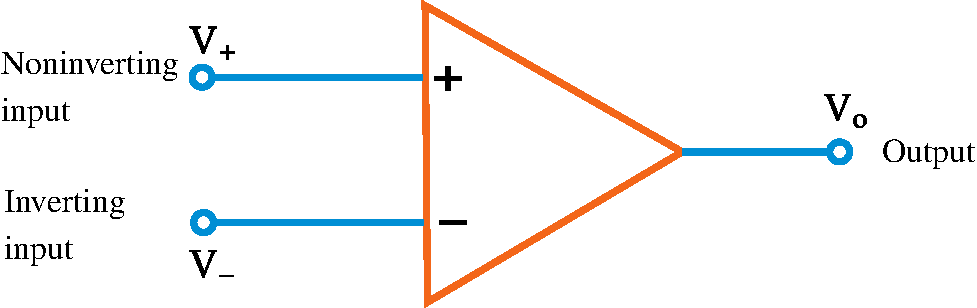
\includegraphics[height=2.2cm,width=7cm]{Opamp schematic}
	\caption{Schematic diagram of an an op-amp}
	\label{Opamp schematic}
\end{figure}
$\left. \right. $\\
 A  schematic diagram of an an op-amp is shown in the figure.\ref{Opamp schematic}. \\
  For  simplicity, power supply and other pin connections are omitted. Since the input differential amplifier stage of the op-amp is designed to be operated in the differential mode, the differential inputs are designated by the $(+)$ and $(-)$ notations. The $(+)$ input is the noninverting input. An ac signal (or dc voltage) applied to this input produces an in-phase (or same polarity) signal at the output. On the other hand, the $(-)$ input is the inverting input because an ac signal (or dc voltage) applied to this input produces an $180^{\circ}$ out-of-phase (or opposite polarity) signal at the output.
   In Figure,
   $$
   \begin{aligned}
   \mathrm{V_{+}}&=\text { Voltage at the noninverting input (volts) } \\
   \mathrm{V_{-}}&=\text { Voltage at the inverting input (volts) } \\
   \mathrm{V_{o}}&=\text { Output voltage (volts) }
   \end{aligned}
   $$
   All these voltages are measured with respect to ground.

  \section{Op-Amp characterestics}
  \subsection{Input offset voltage} 
  
   \begin{figure}[H]
   	\centering
   	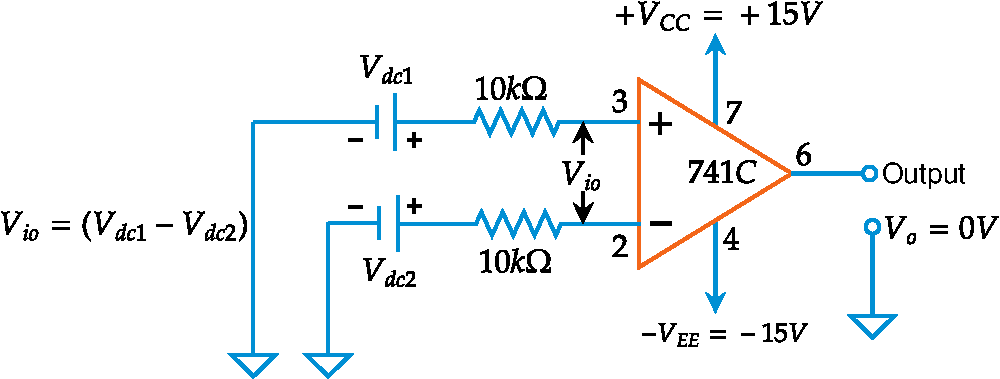
\includegraphics[height=4.5cm,width=11cm]{Input offset voltage}
   	\caption{Defining input offset voltage}
   	\label{Input offset voltage}
   \end{figure}
   \par Input offset voltage is the voltage that must be applied between the two input terminals of an op-amp to null the output, as shown in Figure.\ref{Input offset voltage}. In the figure $V_{\mathrm{dc} 1}$ and $V_{\mathrm{dc} 2}$ are dc voltages and $R_{S}$ represents the source resistance. We denote input offset voltage by $V_{i o}$. This voltage $V_{i o}$ could be positive or negative; therefore, its absolute value is listed on the data sheet. For a $741 \mathrm{C}$ the maximum value of $V_{i o}$ is $6 \mathrm{mV} \mathrm{dc}$. The smaller the value of $V_{i o}$, the better the input terminals are matched. For instance, the $714 \mathrm{C}$ precision op-amp has $V_{i o}=150 \mu \mathrm{V}$ maximum.
   \subsection{Input offset current}
   \begin{figure}[H]
   	\centering
   	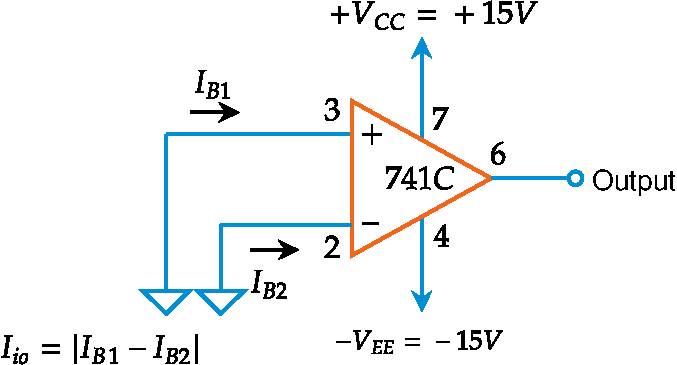
\includegraphics[height=4.5cm,width=8cm]{Input offset current}
   	\caption{Defining input offset current}
   	\label{Input offset current}
   \end{figure}
    The algebraic difference between the currents into the inverting and noninverting terminals is referred to as input offset current, $I_{i o}$. In the form of an equation,
   $$
   I_{i o}=\left|I_{B 1}-I_{B 2}\right|
   $$
   where $I_{B 1}$ is the current into the noninverting input and $I_{B 2}$ is the current into the inverting input.
   \subsection{Input bias current}
   Input bias current, $I_{B}$, is the average of the currents that flow into the inverting and noninverting input terminals of the op-amp. In equation form,
   $$
   I_{B}=\frac{I_{B 1}+I_{B 2}}{2}
   $$
   $I_{B}=500 \mathrm{nA}$ maximum for the $741 \mathrm{C}$, whereas $I_{B}$ for the precision $714 \mathrm{C}$ is $\pm 7 \mathrm{nA} .$ \\
   Note that the two input currents $I_{B 1}$ and $I_{B 2}$ are actually the base currents of the first differential amplifier stage.
   \subsection{Differential input resistance}
   Differential input resistance, $R_{i}$, (often referred to as input resistance) is the equivalent resistance that can be measured at either the inverting or noninverting input terminal with the other terminal connected to oround. For the $741 \mathrm{C}$ the input resistance is a relatively high $2 \mathrm{M} \Omega$.
   \subsection{Common Mode Rejection Ratio (CMRR)}
  \textbf{The common-mode rejection ratio (CMRR) }is defined in several essentially equivalent ways by various manufacturers. Generally, it can be defined as the ratio of the differential voltage gain $A_{d}$ to the common-mode voltage gain $A_{\mathrm{cm}} $ that is,
   \begin{equation}
   \mathrm{CMRR}=\frac{A_{d}}{A_{\mathrm{cm}}}
   \end{equation}
  
   The differential voltage gain $A_{d}$ is the same as the large-signal voltage gain $A$, which is specified on the data sheets; however, the common-mode voltage gain can be determined from  using the equation,
   \begin{equation}
  \mathrm{A}_{\mathrm{cm}}=\frac{V_\mathrm{ocm}}{V_{\mathrm{cm}}}
   \end{equation}
   $$
   \begin{aligned}
   \text{Where ,} V_\mathrm{ocm}&= \text{output common-mode voltage}\\
   V_{\mathrm{cm}}&=\text { input common-mode voltage } \\
   A_{\mathrm{cm}}&=\text { common-mode voltage gain }
   \end{aligned}
   $$
   Generally the $A_{\mathrm{cm}}$ is very small and $A_{d}=A$ is very large, therefore, the $\mathrm{CMK}$ is very large. Being a large value, CMRR is most often expressed in decibels (dB). For the $741 \mathrm{C}$, CMRR is $90 \mathrm{~dB}$ typically.
   \begin{note}
   	  \textbf{Common mode voltage:} When the same voltage is applied to both input terminals, the voltage is called a common-mode voltage, $V_{\mathrm{cm}}$, and the op-amp is said to be operating in the common-mode configuration.
   \end{note}
   \subsection{Output resistance}
   Output resistance, $R_{o}$, is the equivalent resistance that can be measured between the output terminal of the op-amp and the ground (or common point). It is $75 \Omega$ for the $741 \mathrm{C}$ op-amp.
   \subsection{Slew rate}
   Slew rate (SR) is defined as the maximum rate of change of output voltage per unit of time and is expressed in volts per microseconds. In equation form,
   $$
   \mathrm{SR}=\left.\frac{d V_{o}}{\mathrm{dt}}\right|_\mathrm{max} \mathrm{V} / \mu \mathrm{s}
   $$
   Slew rate indicates how rapidly the output of an op-amp can change in response to changes in the input frequency. The slew rate changes with change in voltage gain and is normally specified at unity $(+1)$ gain. The slew rate of an op-amp is fixed; therefore, if the slope requirements of the output signal are greater than the slew rate, then distortion occurs. Thus slew rate is one of the important factors in selecting the op-amp for ac applications, particularly at relatively high frequencies.\\
    One of the drawbacks of the $ 741 \mathrm{C}$ is its low slew rate $(0.5 \mathrm{~V} / \mu \mathrm{s})$ 
   \section{The ideal Op-Amp} 
   An ideal op-amp would exhibit the following electrical characteristics,
   \begin{enumerate}
   	\item  Infinite voltage gain $A$.
   	\item Infinite input resistance $R_{i}$ so that almost any signal source can drive it and there is no loading of the preceding stage.
   	\item Zero output resistance $R_{o}$ so that the output can drive an infinite number of other devices.
   	\item Zero output voltage when input voltage is zero.
   	\item Infinite bandwidth so that any frequency signal from 0 to $\infty \mathrm{Hz}$ can be amplified without attenuation.
   	\item Infinite common-mode rejection ratio so that the output common-mode noise voltage is zero.
   	\item Infinite slew rate so that output voltage changes occur simultaneously with input voltage changes.
   \end{enumerate}
   There are practical op-amps that can be made to approximate some of these characteristics using a negative feedback arrangement.
   \section{ Open-Loop Op-Amp Configurations(Op-Amp without feedback)}
   In the case of amplifiers the term open loop indicates that no connection, either direct or via another network, exists between the output and input terminals. That is, the output signal is not fed back in any form as part of the input signal, and the loop that would have been formed with feedback is open. When connected in open-loop configuration, the op-amp simply functions as a high-gain amplifier. There are three open-loop op-amp configurations,
   \begin{enumerate}
   	\item Differential amplifier
   	\item Inverting amplifier
   	\item Noninverting amplifier.
   \end{enumerate}
   
   \subsection{Differential Amplifier}
   \begin{figure}[H]
   	\centering
   	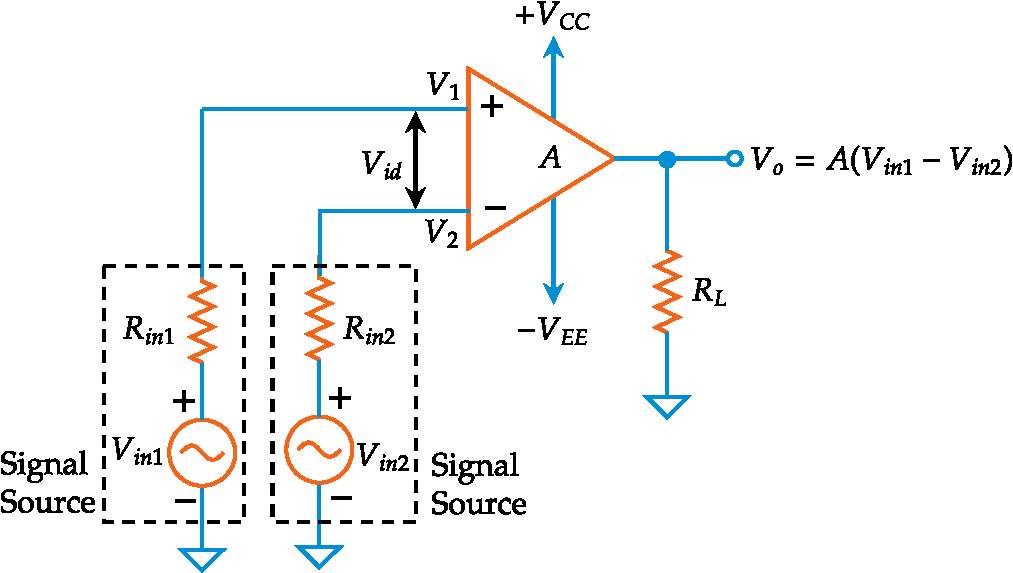
\includegraphics[height=6cm,width=11cm]{Differential Amplifier}
   	\caption{Differential Amplifier}
   	\label{Differential Amplifier}
   \end{figure}
   The differential amplifier circuit amplifies the difference between signals applied to the inputs. The figure.\ref{Differential Amplifier} shows the open-loop differential amplifier in which input signals $V_{\text {in } 1}$ and $V_{\text {in } 2}$ are applied to the positive and negative input terminals. Since the op-amp amplifies the difference between the two input signals, this configuration is called the differential amplifier.\\
   The op-amp is a versatile device because it amplifies both ac and dc input signals. This means that $V_{\text {in } 1}$ and $V_{\text {in } 2}$ could be either ac or dc voltages. The source resistances $R_{\text {in } 1}$ and $R_{\text {in } 2}$ are normally negligible compared to the input resistance $R_{i}$. Therefore, the voltage drops across these resistors can be assumed to be zero, which then implies that $V_{1}=V_{\text {in } 1}$ and $V_{2}=V_{\text {in } 2}$. Then output voltage$V_o$ 
   \begin{equation}
   V_{o}=A\left(V_{\text {in } 1}-V_{\text {in } 2}\right)
   \end{equation}
   Thus, as expected, the output voltage is equal to the voltage gain $A$ times the difference between the two input voltages. Also, notice that the polarity of the output voltage is dependent on the polarity of the input difference voltage $\left(V_{\text {in } 1}-V_{\text {in } 2}\right) .$ In open-loop configurations, gain $\mathbf{A}$ is commonly referred to as \textbf{open-loop gain}. 
   \subsection{Inverting Amplifier}
   In an inverting amplifier only one input is applied and that is to the inverting input terminal. The noninverting input terminal is grounded . Since $V_{1}=0 \mathrm{~V}$, and $V_{2}=V_{\text {in }}$
   \begin{equation}
   V_{o}=-A V_{\mathrm{in}}
   \end{equation} 
   \begin{figure}[H]
   	\centering
   	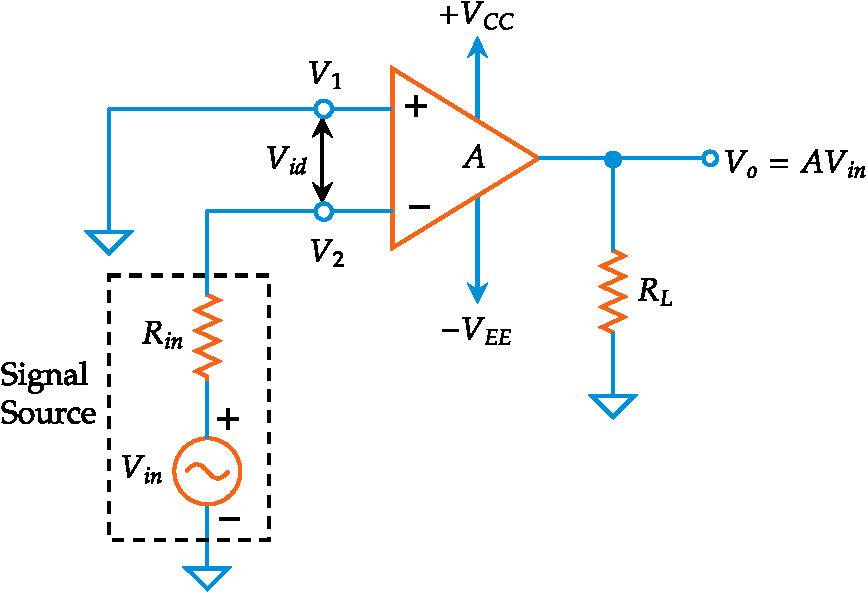
\includegraphics[height=6cm,width=10.5cm]{Inverting Amplifier}
   	\caption{Inverting Amplifier}
   	\label{Inverting Amplifier}
   \end{figure}
   $\left. \right. $\\
   The negative sign indicates that the output voltage is out of phase with respect to input by $180^{\circ}$ or is of opposite polarity. Thus in the inverting amplifier the input signal is amplified by gain $A$ and is also inverted at the output.
   \subsection{Non-inverting Amplifier}
   \begin{figure}[H]
   	\centering
   	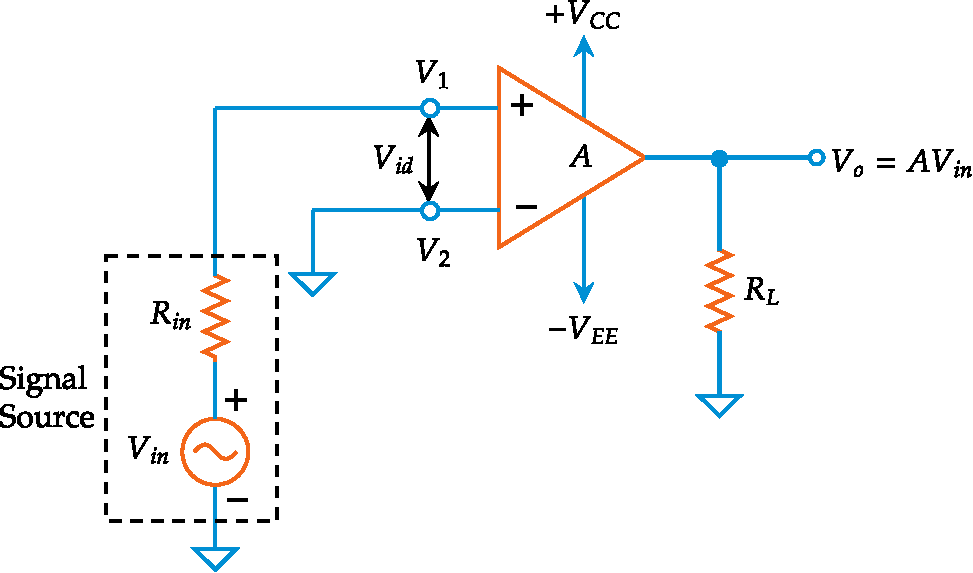
\includegraphics[height=6cm,width=11cm]{Non-inverting Amplifier}
   	\caption{Non-inverting Amplifier}
   	\label{Non-inverting Amplifier}
   \end{figure}
   In Non-inverting configuration the input is applied to the noninverting input terminal, and the inverting terminal is connected to ground. Figure.\ref{Non-inverting Amplifier}  shows the open-loop noninverting amplifier. 
   In the circuit , $ V_{1}=V_{\text {in }}$ and $V_{2}=0 \mathrm{~V}$.
   Therefore,
   \begin{equation}
   V_{o}=A V_{\mathrm{in}}
   \end{equation}
   This means , the output voltage is larger than the input voltage by gain $A$ and is in phase with the input signalIn all three open-loop configurations any input signal (differential or single) that is only slightly greater than zero drives the output to saturation level. This results from the very high gain $(A)$ of the op-amp. Thus, when operated open-loop, the output of the op-amp is either negative or positive saturation or switches between positive and negative saturation levels. For this reason, open-loop op-amp configurations are not used in linear applications.
   \subsection{Drawback of Open-Loop Configuration}
   \begin{itemize}
   	\item Due to the high gain of the Open-loop configuration some portion is clipped out off when the output attempts to exceed the saturation level of the Op-Amp.
   	\item The open-loop voltage gain of the op-amp is not constant.Voltage gain varies with change in temperature and power supply.Which makes opn -loop op-amp unsuitable for linier application.
   	\item The bandwidth(Bnad frequencies for which the gain remains constant) of most open loop op-amp is negligibly small--almost zero.For this reason Open-loop op-amp is impractical in ac application
   \end{itemize}
   For this reasons stated open-loop op-amp is not used in linear applications.Nevertless in certain applications the open-loop op-amp is purposely used as a non linear device.\\
   \section{Negative Feedback Op-Amp}
   \subsection{Benefits of the Negative Feedback}
   \begin{itemize}
   	\item High gain of the open-loop confihuration is controlled by introducing a negative feedback.
   	\item If the signal feedback is of opposite polarity with respect to the input signal the feedback is called negative feedback
   	\item A negative feedback is also known as degenerative feedback because when used it reduces the output voltage amplitude and in turn reduces the voltage gain.
   	\item When used in amplifiers negative feedback stabilizes the gain,increases the bangwidth and changes the input output resistance.
   	\item Negative feedback decreases harmonic or non linear distortion.
   	\item Negative feedback also reduces the efffect of variation in temperature and supply voltages on the output of the op-amp.
   \end{itemize}
   \subsection{Inverting Amplifier}
   \begin{figure}[H]
   	\centering
   	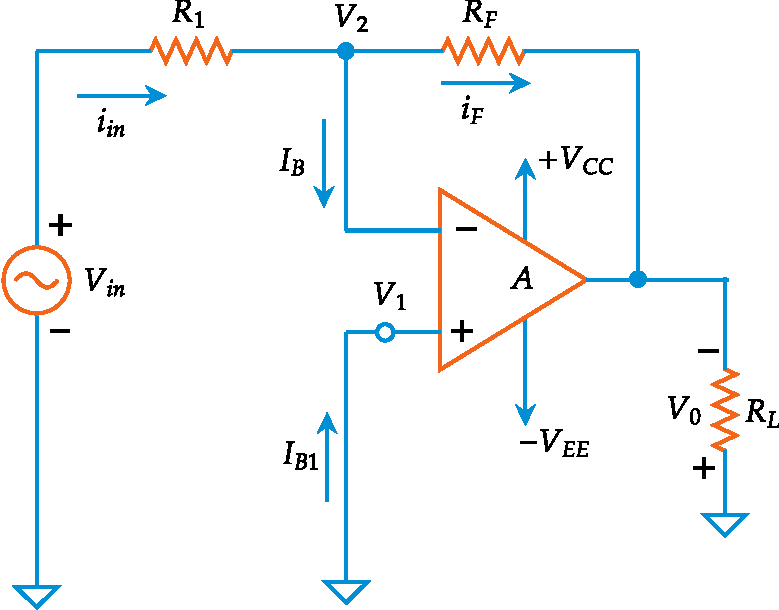
\includegraphics[height=6cm,width=8cm]{NF Inverting Amplifier}
   	\caption{Negative feedback Inverting Amplifier}
   	\label{NF Inverting Amplifier}
   \end{figure}
   Figure shows the voltage-shunt feedback amplifier using an op-amp. The input voltage drives the inverting terminal, and the amplified as well as inverted output signal is also applied to the inverting input via the feedback resistor $R_{F}$. This arrangement forms a negative feedback because any increase in the output signal results in a feedback signal into the inverting input, causing a decrease in the output signal.\\
   Note that the noninverting terminal is grounded, and the feedback circuit has only one resistor $R_{F}$. However, an extra resistor $R_{1}$ is connected in series with the input signal source $V_{\text {in }}$.
   \subsubsection{Closed Loop Voltage Gain}  
   The closed-loop voltage gain $A_{F}$ of the voltage-shunt feedback amplifier can be obtained by writing Kirchhoff's current equation at the input node $V_{2}$  as follows,
   \begin{align*}
   i_{\text {in }}&=i_{F}+I_{B}
   \intertext{Since  R is very large the input bias current  $I_{B}$  is negligibly small}
   i_{\mathrm{in}} &\cong i_{F} \\
   \frac{V_{\text {in }}-V_{2}}{R_{1}}&=\frac{V_{2}-V_{o}}{R_{F}}\\
   \text{However we know } V_{1}-V_{2}&=\frac{V_{o}}{A}\\
   \text{Since $V_{1}=0 \mathrm{~V}$ } V_{2}&=-\frac{V_{o}}{A}
   \intertext{ Substituting this value of $V_{2}$ in above Equation  and rearranging, we get,}
   \frac{V_{\text {in }}+V_{o} / A}{R_{1}} &=\frac{-\left(V_{o} / A\right)-V_{o}}{R_{F}} \\
   A_{F} &=\frac{V_{o}}{V_{\text {in }}}\\&=-\frac{A R_{F}}{R_{1}+R_{F}+A R_{1}} \quad \text { (exact) }
   \end{align*}
   The negative sign in Equation  indicates that the input and output signals are out of phase by $180^{\circ}$ (or of opposite polarities). In fact, because of this phase inversion, the configuration in Figure is commonly called an inverting amplifier with feedback.
   Since the internal gain $A$ of the op-amp is very large (ideally infinity), $A R_{1} \gg R_{1}+R_{F}$. This means that Equation can be rewritten as,
   \begin{equation}
   A_{F}=\frac{V_{o}}{V_{\text {in }}}=-\frac{R_{F}}{R_{1}} \quad \text { (ideal) }
   \end{equation}
   \begin{center}
   	\framebox{
   		\parbox[t][0.75cm]{4cm}{
   			
   			\addvspace{0.2cm} \centering 
   			
   			$ A_{F}=\frac{V_{o}}{V_{\text {in }}}=-\frac{R_{F}}{R_{1}}$} }
   \end{center}
   \begin{note}
   	\begin{itemize}
   		\item 	Since the ratio $\frac{R_F}{R_1}$ can be set in to less than 1 it can use for more applications that cant be used by a non inverting amplifier.
   		\item \textbf{The inverting input terminal is at virtual ground}\\
   		$$V_{id}=\frac{V_o}{A}$$ Since the value of A is very high,$V_{id}$ is approximately zero.So the potential at each terminal should be same. Here the therminal $v_1$ is grounded.The voltage at $V_2$ should be also zero.Therfore the the terminal $V_2$ is said to be grounded virtually.
   		This idea can be used to find the voltage gain easily.
   		From the circuit ,
   		\begin{align*}
   		i_{in}&=i_f
   		\frac{V_{in}-V_2}{R_1}&=\frac{V_2-V_o}{R_F}
   		\end{align*}
   		
   		$$V_1=V_2=0$$
   		$$\frac{V_{in}}{R_1}=-\frac{V_o}{R_F}$$
   		$$A_F=\frac{V_o}{V_{in}}=-\frac{R_F}{R_1}$$
   		This is the same result that we got before.
   	\end{itemize}
   \end{note}
   \subsubsection{Input resistance}
   The input resistance with feedback can be written as \\
   $$R_{iF}=R_1+\frac{R_F}{1+A}\vert\vert R_i$$
   Since $R_i$ and A are very large.\\
   $$\frac{R_F}{1+A}\vert\vert R_i\approx 0\Omega$$
   Then 
   $$R_{iF}=R_1$$
   \subsubsection{Output resistance}
   $$R_{oF}=\frac{R_0}{1+AB}$$
   Where,\\
   $R_O$=Output resistance of the op-amp with out feedback\\
   A= Open-loop voltage gain of the op-amp\\
   B= Gain of the feedback circuit\\
   $$B=\frac{R_1}{R_1+R_F}$$
   \subsubsection{Bandwidth}
   We know that the gain of the amplifier with feedback is less than the gain without feedback.Therfore the bandwidth of the amplifier with feedback $f_F$ must be larger than that without the feedback.
   $$f_F=f_0(1+AB)$$
   Where $f_0$=Break frequency of the op-amp.\\
   which can be defined as 
   \begin{align*}
   f_0&=\frac{\text{Unit gain bandwidth}}{\text{Open-loop voltage gain}}\\
   &=\frac{UGB}{A}\\
   f_F&=\frac{UGB}{A}(1+AB)\\
   f_F&=\frac{UGB(K)}{A}\\
   \text{Where, } K&=\frac{R_F}{R_1+R_F}\\
   A_F&=\frac{AK}{1+AB}
   \end{align*}
   
   \subsection{Non-inverting amplifier}
   The noninverting amplifier with feedback (or closed-loop noninverting amplifier)called so  because it uses feedback, and the input signal is applied to the noninverting input terminal of the op-amp.
   \begin{figure}[H]
   	\centering
   	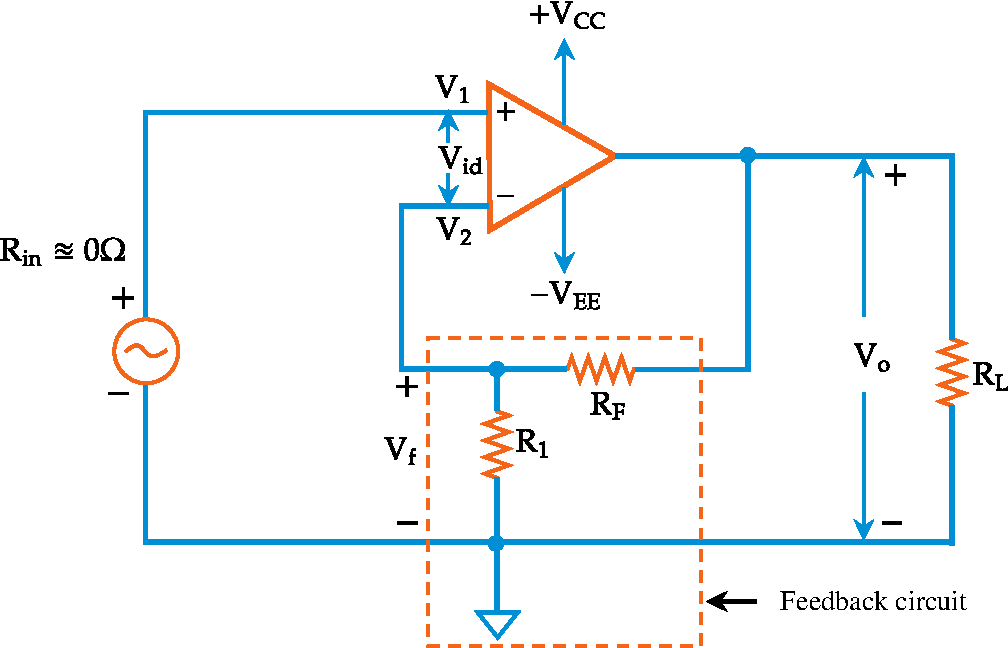
\includegraphics[height=6.5cm,width=10cm]{Non Inverting Amplifier}
   	\caption{Voltage series Non Inverting Amplifier}
   	\label{Non Inverting Amplifier}
   \end{figure}
   Important terms for the voltage-series feedback amplifier:
   \begin{align*}
   V_{\text {in }}&= \text{Input voltage.}\\
   V_{\text {f }}&=\text{Feedback voltage.}\\
   V_{\text {id }}&=\text{Difference input voltage.}\\
   \text{Open-loop voltage gain (or gain without feedback) } A&=\frac{V_{o}}{V_{i d}}\\
   \text{Here, } V_{i d}&=V_{\text {in }}-V_{f}\\
   \text{Closed-loop voltage gain (or gain with feedback) } A_{F}&=\frac{V_{o}}{V_{\text {in }}}\\
   \text{Gain of the feedback circuit } B&=\frac{V_{f}}{V_{o}}
   \end{align*}
   
   \subsubsection{Voltage gain}
   As defined previously, the closed-loop voltage gain is,
   \begin{align*}
   A_{F}&=\frac{V_{o}}{V_{\mathrm{in}}}\\
   \text{But, } V_{o}&=A\left(V_{1}-V_{2}\right)\\
   V_{1}&=V_{\text {in }} \\
   V_{2}&=v_{f}=\frac{R_{1} V_{o}}{R_{1}+R_{F}} \quad \text { since } R_{i} \gg R_{1}\\
   \text{Therefore, } V_{o}&=A\left(V_{\text {in }}-\frac{R_{1} V_{o}}{R_{1}+R_{F}}\right)\\
   \text{Rearranging we get, }V_{o}&=\frac{A\left(R_{1}+R_{F}\right) V_{\mathrm{in}}}{R_{1}+R_{F}+A R_{1}}\\
   A_{F}&=\frac{V_{o}}{V_{\text {in }}}=\frac{A\left(R_{1}+R_{F}\right)}{R_{1}+R_{F}+A R_{1}} \quad \text { (exact) }
   \intertext{Generally, $A$ is very large (typically $10^{5}$ ). Therefore,}
   A R_{1} &\gg\left(R_{1}+R_{F}\right) \quad \text { and } \quad\left(R_{1}+R_{F}+A R_{1}\right) \cong A R_{1}\\
   \text{Thus, } A_{F}&=\frac{V_{o}}{V_{\text {in }}}\\&=1+\frac{R_{F}}{R_{1}} \quad \text { (ideal) }
   \end{align*}
   
   \begin{note}
   	\begin{itemize}
   		\item \textbf{$A_F$ in terms of B}\\\\
   		Feedback circuit gain B is the ratio of $V_f$ and $V_o$ 
   		\begin{align*}
   		B&=\frac{V_f}{V_o}\\
   		&=\frac{R_1}{R_1+R_F}\\
   		A_F&=\frac{1}{B}
   		\end{align*}
   		
   		\item \textbf{$A_F$ in terms of A and B.}
   		\begin{align*}
   		A_{F}&=\frac{V_{o}}{V_{\text {in }}}\\&=\frac{A\left(R_{1}+R_{F}\right)}{R_{1}+R_{F}+A R_{1}}\\
   		A_{F}&=\frac{A\left(\frac{R_{1}+R_{F}}{R_{1}+R_{F}}\right)}{\frac{R_{1}+R_{F}}{R_{1}+R_{F}}+\frac{A R_{1}}{R_{1}+R_{F}}}\\
   		\text{Using Equation for B, } A_{F}&=\frac{A}{1+A B} \\ 
   		\text{Where, } A_{F}&= \text{ closed-loop voltage gain}\\
   		A &=\text { open-loop voltage gain } \\
   		B &=\text { gain of the feedback circuit } \\
   		A B &=\text { loop gain }
   		\end{align*}
   	\end{itemize}
   \end{note}
   \subsubsection{Difference Input Voltage Ideally Zero.}
   \begin{align*}
   \text{We know } 
   v_{i d}&=\frac{V_{o}}{A}\\
   \text{Since $A$ is very large}&\text{ (ideally infinite), }
   v_{i d} \cong 0\\
   V_{1} &\cong V_{2}\\
   \text{Then, } V_{1} &=V_{\mathrm{in}} \\
   V_{2} &=v_{f} \\
   &=\frac{R_{1} V_{o}}{R_{1}+R_{F}}
   \intertext{	Substituting these values of $V_{1}$ and $V_{2}$ , we get}
   V_{\text {in }}&=\frac{R_{1} V_{o}}{R_{1}+R_{F}}\\
   \text{i.e., } A_{F}&=\frac{V_{o}}{V_{\text {in }}}\\&=1+\frac{R_{F}}{R_{1}}
   \end{align*}
   \subsubsection{Input resistance with feedback.}
   $R_i$ is the input resistance of the op-amp and $R_{iF}$ is the input resistance of the amplifier with feedback.The input resistance with feedback is defined as ,
   \begin{align*}
   R_{i F} &=\frac{V_{\mathrm{in}}}{i_{\mathrm{in}}} \\
   &=\frac{V_{\mathrm{in}}}{v_{i d} / R_{i}}\\
   \text{However we know ,} V_{i d}&=\frac{V_{o}}{A} \quad \text { and } \quad V_{o}=\frac{A}{1+A B} V_{\mathrm{in}}\\
   \text{Therefore, }
   R_{i F} &=R_{i} \frac{V_{\mathrm{in}}}{v_{t} / A} \\
   &=A R_{i} \frac{V_{\mathrm{in}}}{A V_{\mathrm{in}} /(1+A B)} \\
   R_{i F}&=R_{i}(1+A B)
   \end{align*}
   
   \subsubsection{Output resistance with feedback}
   $$R_{oF}=\frac{R_0}{1+AB}$$
   \subsubsection{Bandwidth}
   \begin{equation}
   \mathrm{UGB}=(A)\left(f_{o}\right) \label{Feedback Bandwidth 1}
   \end{equation}
   Where $A=$ open-loop voltage gain
   $f_{o}=$ break frequency of an op-amp
   or, alternatively, only for a single break frequency op-amp,
   \begin{equation}
   \mathrm{UGB}=\left(A_{F}\right)\left(f_{F}\right)\label{Feedback Bandwidth 2}
   \end{equation}
   Where $A_{F}=$ closed-loop voltage gain
   $f_{F}=$ bandwidth with feedback
   Therefore, equating Equations .\ref{Feedback Bandwidth 1} and \ref{Feedback Bandwidth 2},
   $(A)\left(f_{o}\right)=\left(A_{F}\right)\left(f_{F}\right)$
   \begin{equation}
   f_{F}=\frac{(A)\left(f_{o}\right)}{A_{F}}\label{Feedback Bandwidth 3}
   \end{equation}
   However, for the noninverting amplifier with feedback,
   \begin{align}
   A_{F}&=\frac{A}{1+A B}
   \intertext{Therefore, substituting the value of $A_{F}$ in Equation \ref{Feedback Bandwidth 3}, we get}
   f_{F}&=\frac{(A)\left(f_{o}\right)}{A /(1+A B)}\\
   f_{F}&=f_{o}(1+A B)
   \end{align}
   
   \subsection{Differential amplifier}
   \begin{figure}[H]
   	\centering
   	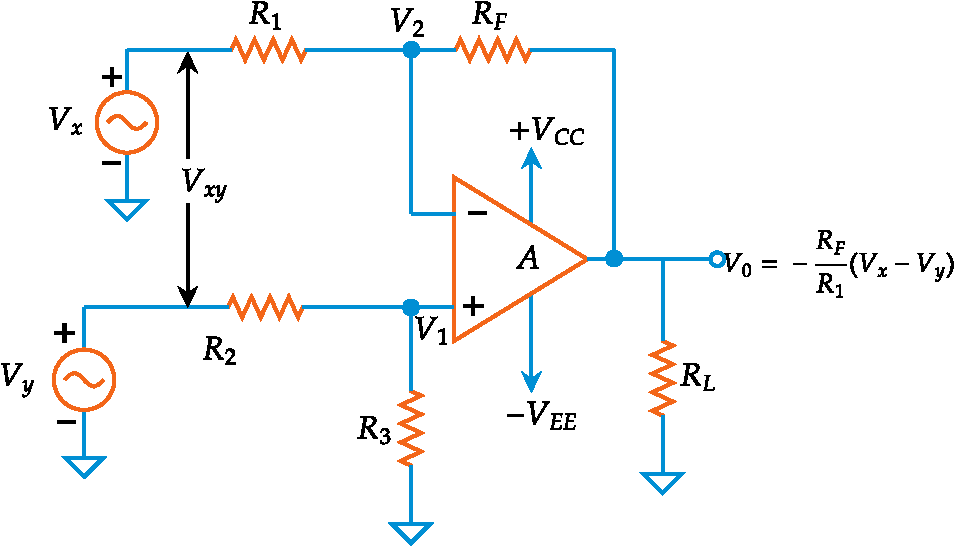
\includegraphics[height=5.7cm,width=10cm]{diagram-20211125-crop}
   	\caption{}
   	\label{}
   \end{figure}
   A differential amplifier is a type of electronic amplifier that amplifies the difference between two input voltages but suppresses any voltage common to the two inputs. It is a combination of inverting and noninverting amplifiers. That is, when $V_{x}$ is reduced to zero the circuit is a noninverting amplifier, whereas the circuit is an inverting amplifier when input $V_{y}$ is reduced to zero.
   \subsubsection{Voltage Gain}
   The circuit in Figure  has two inputs, $V_{x}$ and $V_{y}$; we will, therefore, use the superposition theorem in order to establish the relationship between inputs and output. When $V_{y}=0 \mathrm{~V}$, the configuration becomes an inverting amplifier; hence the output due to $V_{x}$ only is
   \begin{equation}
   V_{o x}=-\frac{R_{F}\left(V_{x}\right)}{R_{1}}
   \end{equation}
   
   Similarly, when $V_{x}=0 \mathrm{~V}$, the configuration is a noninverting amplifier having a voltage-divider network composed of $R_{2}$ and $R_{3}$ at the noninverting input. Therefore,
   \begin{equation}
   V_{1}=\frac{R_{3}\left(V_{y}\right)}{R_{2}+R_{3}}
   \end{equation}
   
   and the output due to $V_{y}$ then is
   \begin{align*}
   V_{o y}&=\left(1+\frac{R_{F}}{R_{1}}\right) V_{1}
   \text{That is, } V_{o y}&=\frac{R_{3}}{R_{2}+R_{3}}\left(\frac{R_{1}+R_{F}}{R_{1}}\right) V_{y}
   \intertext{ Since $R_{1}=R_{2}$ and $R_{F}=R_{3}$, }
   V_{o y}&=\frac{R_{F}\left(V_{y}\right)}{R_{1}}\\
   V_{o}&=V_{o x}+V_{o y} \\
   V_{o}&=-\frac{R_{F}}{R_{1}}\left(V_{x}-V_{y}\right)\\&=-\frac{R_{F}\left(V_{x y}\right)}{R_{1}}\\
   \text{Or the voltage gain }
   A_{D}&=\frac{V_{o}}{V_{x y}}=-\frac{R_{F}}{R_{1}}\quad ;\quad  A_{D}=-\frac{R_{F}}{R_{1}}
   \end{align*}
   
   Note that the gain of the differential amplifier is the same as that of the inverting amplifier.
   \section{Comparison of Inverting and Non Inverting Amplifier}
   
   \begin{table}[H]
   	\centering
   	\renewcommand*{\arraystretch}{1.9}
   	\arrayrulecolor{ocre}
   	\begin{tabular}{|p{4cm}|p{5.5cm}|p{5.5cm}|}
   		\hline
   		
   		\textbf{	Parameter}\newline  &\textbf{Noninverting Amplifier}\newline &\textbf{Inverting Amplifier}\newline\\\hline
   		Voltage gain& $\begin{aligned}
   		A_{F}  &=\frac{A\left(R_{1}+R_{F}\right)}{R_{1}+R_{F}+A R_{1}} \text { (exact) }\\
   		&=\frac{A}{1+A B}\\
   		&=1+\frac{R_{F}}{R_{1}} \text { (ideal) }
   		\end{aligned}$  & $\begin{aligned}
   		A_{F}  &=\frac{-A R_{F} .}{R_{1}+R_{F}+A R_{1}} \text { (exact) }\\
   		&=\frac{-A K}{1+A B}, \text { where } K=\frac{R_{F}}{R_{1}+R_{F}}\\
   		&=-\frac{R_{F}}{R_{1}} \text { (ideal) }
   		\end{aligned}$ \\\hline
   		Gain of the feedback circuit& $\left. \right.B=\frac{R_{1}}{R_{1}+R_{F}}$ & $\left. \right.B=\frac{R_{1}}{R_{1}+R_{F}}$\\\hline
   		Input resistance& $\left. \right. R_{i F}=R_{i}(1+A B)$ & $\left. \right. R_{i F}=R_{1}+\left(\frac{R_{F}}{1+A} \| R_{i}\right)$ \\\hline
   		Output resistance  & $ \left. \right. R_{o F}=\frac{R_{o}}{1+A B} $&$\left. \right. R_{o F}=\frac{R_{o}}{1+A B}$ \\\hline
   		Bandwidth&$\begin{aligned}
   		f_{F}&=f_{o}(1+A B)\\
   		f_{F}&=\frac{\mathrm{UGB}}{A_{F}}
   		\end{aligned}$ &$\begin{aligned}
   		f_{F}&=f_{o}(1+A B)\\
   		f_{F}&=\frac{(\mathrm{UGB})(K)}{A_{F}}
   		\end{aligned}$ \\\hline
   		Total output offset voltage&$\left. \right.V_{ooT}=\frac{\pm V_{Sat}}{1+AB}$ &$\left. \right.V_{ooT}=\frac{\pm V_{Sat}}{1+AB}$ \\\hline
   	\end{tabular}
   \end{table}
   \section{General Linear Application}
   Inverting, non inverting and differential configurations are useful in such applications as summing, scaling and averaging amplifiers.
   \subsection{Inverting Configuration}
   \subsection{Summing, Scaling and Averaging Amplifiers}
   The figure shows the inverting configuration with three inputs $V_a,V_b and V_c$.Depending up on the feedback resistors and $R_a,R_b $ and $R_c$ the circuit can be used as a summing amplifier, scaling amplifier and an averaging amplifier.
   \begin{figure}[H]
   	\centering
   	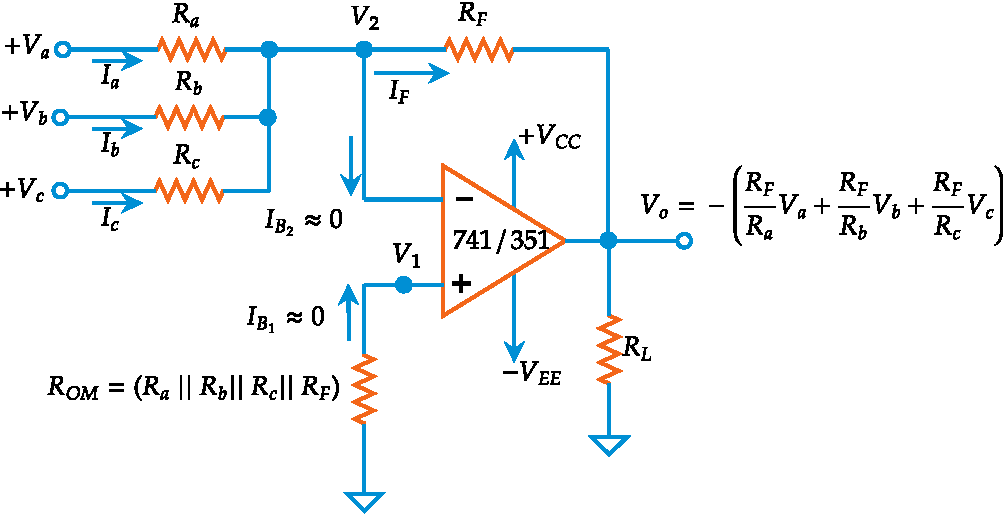
\includegraphics[height=6cm,width=11.2cm]{SSA amplifier}
   	\caption{Inverting configuration with three inputs}
   	\label{SSA amplifier}
   \end{figure}
   The circuit function can be verified by examining the expression for the output voltage $V_o$ Which is obtained by Kirchoff's current equation written at node $V_2$. Then ,
   \begin{align}
   I_a+I_b+I_c&=I_B+I_Fb 
   \intertext{$\because R_i$ and $A$ of the op-amp are ideally infinity. } I_B&=0 \text{ and } V_1=V_2=0V\\
   \frac{V_a}{R_a}+\frac{V_b}{R_b}+\frac{V_c}{R_c}&=-\frac{V_o}{R_F}\\
   V_o&=-\left( \frac{R_F}{R_a}V_a+\frac{R_F}{R_a}V_b+\frac{R_F}{R_C}V_C\right)\label{SSA Amplifier 1}
   \end{align}
   
   \subsubsection{Summing Amplifier}
   In the figure.\ref{SSA amplifier} ,if $ R_{a}=R_{b}=R_{c}=R$, then Equation  can be rewritten as
   \begin{equation}
   V_{o}=-\frac{R_{F}}{R}\left(V_{a}+V_{b}+V_{c}\right)
   \end{equation}
   Then the output voltage is equal to the negative sum of all the inputs times the gain of the circuit $R_{F} / R$; hence the circuit is called a summing amplifier. Obviously, when the gain of the circuit is 1 , that is, $R_{a}=R_{b}=R_{c}=R_{F}$, the output voltage is equal to the negative sum of all input voltages. Thus,
   \begin{equation}
   V_{o}=-\left(V_{a}+V_{b}+V_{c}\right)
   \end{equation}
   \subsubsection{Scaling or Weighted Amplifier}
   If each input voltage is amplified by a different factor, in other words, weighted differently at the output, the circuit in figure.\ref{SSA amplifier} is then called a scaling or weighted amplifier. This condition can be accomplished if $R_{a}, R_{b}$, and $R_{c}$ are different in value. Thus the output voltage of the scaling amplifier is,
   \begin{equation}
   V_{o}=-\left(\frac{R_{F}}{R_{a}} V_{a}+\frac{R_{F}}{R_{b}} V_{b}+\frac{R_{F}}{R_{c}} V_{c}\right)
   \end{equation}
   Where, $\frac{R_{F}}{R_{a}} \neq \frac{R_{F}}{R_{b}} \neq \frac{R_{F}}{R_{c}}$
   \subsubsection{Average circuit}
   The circuit of figure.\ref{SSA amplifier}  can be used as an averaging circuit, in which the output voltage is equal to the average of all the input voltages. This is accomplished by using all input resistors of equal value, $R_{a}=R_{b}=R_{c}=R$. In addition, the gain by which each input is amplified must be equal to 1 over the number of inputs; that is,
   $$
   \frac{R_{F}}{R}=\frac{1}{n}
   $$
   Where $n$ is the number of inputs.
   Thus, if there are three inputs , we want $R_{F} / R=1 / 3$. Consequently,from equation. \ref{SSA Amplifier 1}
   \begin{equation}
   V_{o}=-\left(\frac{V_{a}+V_{b}+V_{c}}{3}\right)
   \end{equation}
   \subsection{Non-Inverting Configuration}
   \subsection{Summing and Averaging Amplifiers  }
   \begin{figure}[H]
   	\centering
   	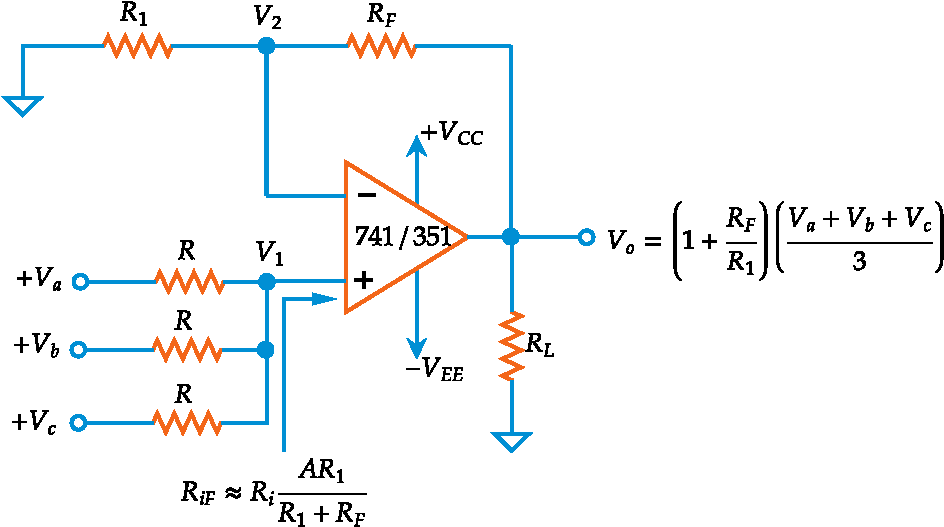
\includegraphics[height=6cm,width=11.2cm]{SSA Non inverting}
   	\caption{Non-Inverting configuration with three inputs}
   	\label{SSA Non inverting}
   \end{figure} 
   If  input voltage source and resistors are connected to the non-inverting terminal , the circuit can be used as a summing or averaging amplifier through the selection of appropriate values of resistors ,i.e.,  $R_1$ and $R_F$\\
   We know that the input resistance $R_{if}$ of the non-inverting amplifier is very large, by using the superposition theorem the voltage $V_1$ at the non-inverting terminal is,
   \begin{align}
   V_{1}&=\frac{R / 2}{R+R / 2} V_{a}+\frac{R / 2}{R+R / 2} V_{b}+\frac{R / 2}{R+R / 2} V_{c} \\
   V_{1}&=\frac{V_{a}}{3}+\frac{V_{b}}{3}+\frac{V_{c}}{3}\\&=\frac{V_{a}+V_{b}+V_{c}}{3}
   \intertext{Hence the output voltage $V_{o}$ is}
   V_{o} &=\left(1+\frac{R_{F}}{R_{1}}\right) V_{1} \\
   &=\left(1+\frac{R_{F}}{R_{1}}\right) \frac{V_{a}+V_{b}+V_{c}}{3}
   \end{align}
   \subsubsection{Averaging amplifier}
   \begin{equation}
   V_o=\left(1+\frac{R_{F}}{R_{1}}\right) \frac{V_{a}+V_{b}+V_{c}}{3}\label{Non inverting Averaging amplifier}
   \end{equation}
   Equation. \ref{Non inverting Averaging amplifier} shows that the output voltage is equal to the average of all input voltages times the gain of the circuit $\left(1+R_{F} / R_{1}\right)$, hence the name averaging amplifier. Depending on the application requirement, the gain $\left(1+R_{F} / R_{1}\right)$ can be set to a specific value. Obviously, if the gain is 1 , the output voltage will be equal to the average of all input voltages.\\
   Note that there are two basic differences between this averaging amplifier and that using the inverting configuration\\
   1. No sign change or phase reversal occurs between the average of the inputs and output.\\
   2. The noninverting input voltage $V_{1}$ is the average of all inputs, whereas in the inverting averaging amplifier the output is the average of all inputs, with a negative sign.
   \subsubsection{Summing amplifier}
   In the equation. \ref{Non inverting Averaging amplifier}  if the gain $\left(1+\frac{R_{F}}{R_{1}}  \right)$ is equal to the number of inputs, the output voltage becomes equal to the sum of all input voltages. That is, if $\left(1+\frac{R_{F}}{R_{1}}  \right)$
   \begin{equation}
   V_{o}=V_{a}+V_{b}+V_{c}
   \end{equation}
   Hence the circuit is called a noninverting summing amplifier.
   \subsection{Differential Configuration}
   \subsection{A Substractor and Summing Amplifier}
   Using a basic differential op-amp configuration a substractor and a summimg amplifier may be constructed .
   \subsubsection{A Subtractor}
   \begin{figure}[H]
   	\centering
   	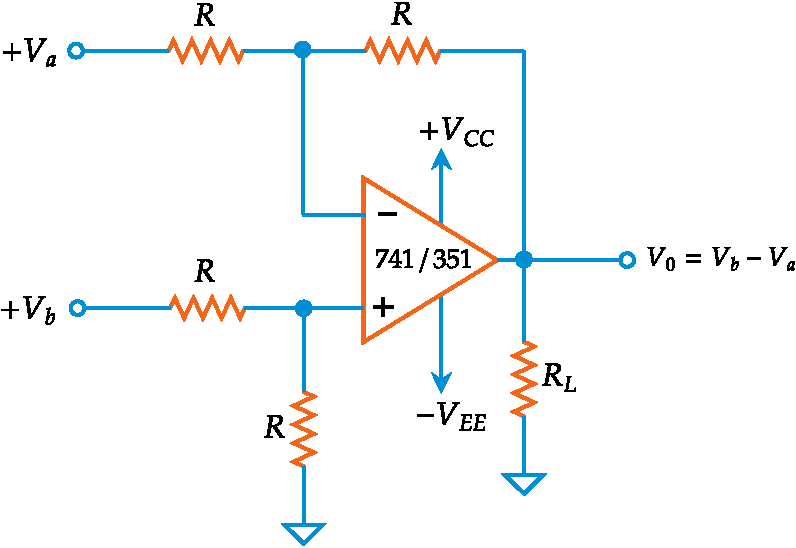
\includegraphics[height=6cm,width=9.8cm]{Subtractor}
   	\caption{Basic differential amplifier as a subtractor}
   	\label{Subtractor}
   \end{figure}
   A basic amplifier can be used as a substractor as shown in the figure. In the figure the input signal can be scaled to desired value by selecting appropriate value for the external resisistors :When this is done the circuit is reffered to a scalling amplifier. However in the figure the external resistors are equal in value,so the gain of the amplifier is equal to one.\\
   The output voltage of the differential amplifier with a gain of 1 is ,
   \begin{align}
   V_o&=-\frac{R}{R}(V_a-V_b)\\
   \text{i.e., }V_o&=V_b-V_a
   \end{align}
   Thus output voltage $V_o$ is equal to the voltage $V_b$ applied to the non-inverting terminal minus the voltage $V_a$ applied to the inverting terminal. Hence the circuit is called a subtractor.
   \subsubsection{Summing Amplifier}
   \begin{figure}[H]
   	\centering
   	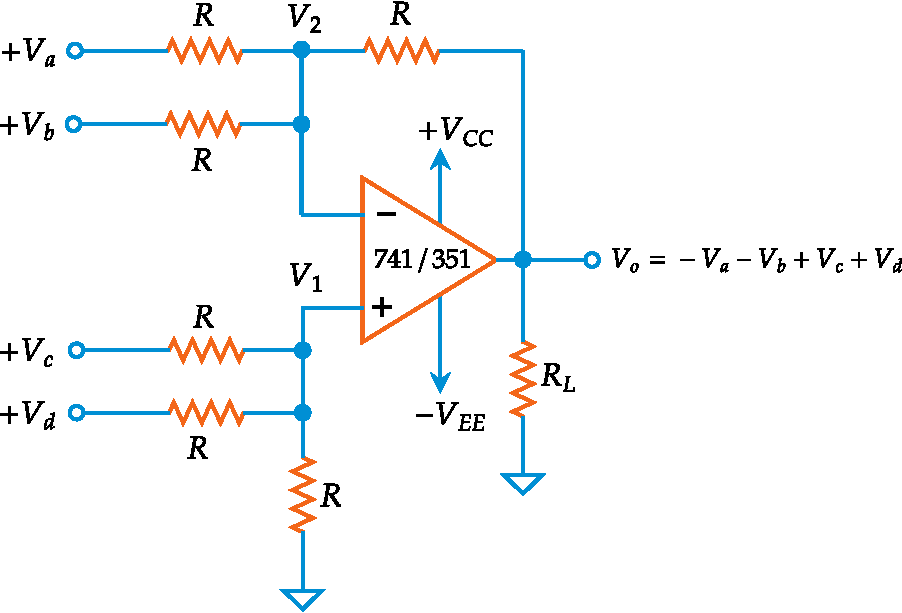
\includegraphics[height=6.5cm,width=10.5cm]{Differential Summing amplifier}
   	\caption{Summing amplifier Using Differential Amplifier}
   	\label{Differential Summing amplifier}
   \end{figure}
   A four input summing amplifier may be constructed using the basic different amplifier if two additional input sources are connected, one each to the inverting and noninverting input terminals through resistor $R$\\ The output voltage equation for this circuit can be obtained by using the superposition theorem. For instance, to find the output voltage due to $V_{a}$ alone, reduce all other input voltages $V_{b}, V_{c}$, and $V_{d}$ to zero . In 
   fact, this circuit is an inverting amplifier in which the inverting input is at virtual ground $\left(V_{2}=0 \mathrm{~V}\right)$. Therefore, the output voltage is
   $$V_{o a}=-\frac{R}{R} V_{a}=-V_{a}$$
   Similarly, the output voltage due to $V_{b}$ alone is
   $$
   V_{o b}=-V_{b}
   $$
   Now if input voltages $V_{a}, V_{b}$, and $V_{d}$ are set to zero, the circuit in Figure  becomes a noninverting amplifier in which the voltage $V_{1}$ at the noninverting input is
   $$V_{1}=\frac{R / 2}{R+R / 2} V_{c}=\frac{V_{c}}{3}$$
   This means that the output voltage due to $V_{c}$ alone is
   $$
   V_{o c}=\left(1+\frac{R}{R / 2}\right) V_{1}=(3)\left(\frac{V_{c}}{3}\right)=V_{c}
   $$
   Similarly, the output voltage due to input voltage $V_{d}$ alone is
   $$
   V_{o d}=V_{d}
   $$
   Thus by using the superposition theorem the output voltage due to all four input voltages is given by
   $$
   \begin{aligned}
   V_{o} &=V_{o a}+V_{o b}+V_{o c}+V_{o d} \\
   &=-V_{a}-V_{b}+V_{c}+V_{d}
   \end{aligned}
   $$
   Notice that the output voltage is equal to the sum of the input voltages applied to the noninverting terminal plus the negative sum of the input voltages applied to the inverting terminal.
   \section{The Integrator}
   \begin{figure}[H]
   	\centering
   	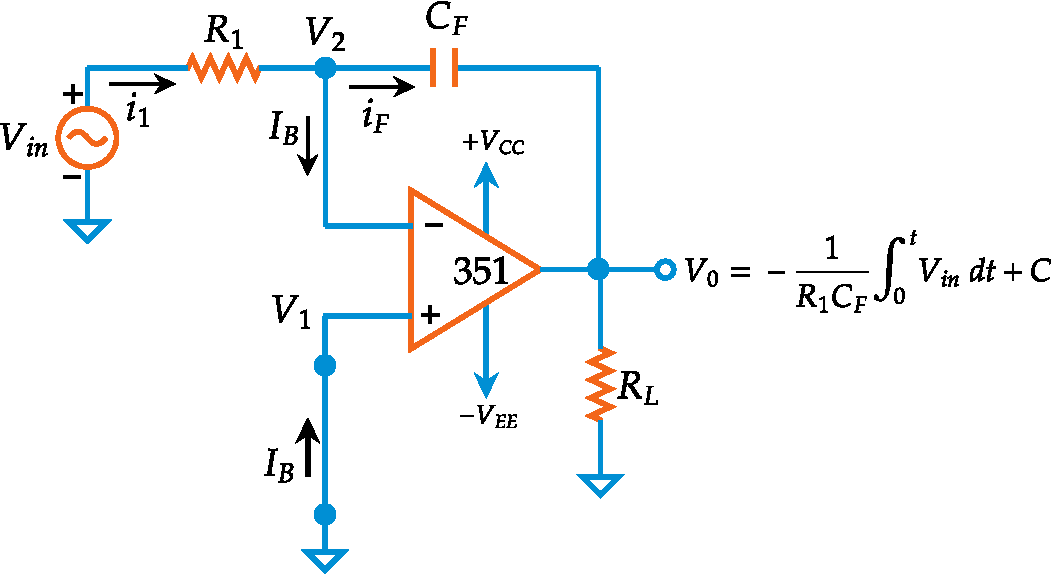
\includegraphics[height=6cm,width=11cm]{diagram-20211126-crop}
   	\caption{}
   	\label{}
   \end{figure}
   A circuit in which the output voltage waveform is the integral of the input voltage waveform is the integrator or the integration amplifier. Such a circuit is obtained by using a basic inverting amplifier configuration if the feedback resistor $R_{F}$ is replaced by a capacitor $C_{F}$
   The expression for the output voltage $V_{o}$ can be obtained by writing Kirchhoff's current equation at node $V_{2}$ ,
   \begin{align*}
   i_{1}&=I_{B}+i_{F}
   \intertext{Since $I_{B}$ is negligibly small,}
   i_{1} &\cong i_{F}
   \intertext{Recall that the relationship between current through and voltage across the capacitor is,}
   i_{c}&=C \frac{d v_{c}}{d t}\\
   \text{ Therefore, } \frac{V_{\mathrm{in}}-V_{2}}{R_{1}}&=C_{F}\left(\frac{d}{d t}\right)\left(V_{2}-V_{o}\right)
   \intertext{However, $V_{1}=V_{2} \cong 0$ because $A$ is very large. Therefore,}
   \frac{V_{\mathrm{in}}}{R_{1}}&=C_{F} \frac{d}{d t}\left(-V_{o}\right)
   \intertext{The output voltage can be obtained by integrating both sides with respect to time:}
   \int_{0}^{t} \frac{V_{\text {in }}}{R_{1}} d t &=\int_{0}^{t} C_{F} \frac{d}{d t}\left(-V_{o}\right) d t \\
   &=C_{F}\left(-V_{o}\right)+\left.V_{o}\right|_{t=0}\\
   \text{Therefore, } V_{o}&=-\frac{1}{R_{1} C_{F}} \int_{0}^{t} V_{\text {in }} d t+C
   \end{align*}
   Where $C$ is the integration constant and is proportional to the value of the output voltage $V_{o}$ at time $t=0$ seconds.
   \begin{note}
   	\begin{itemize}
   		\item The output voltage is directly proportional to the negative integral of the input voltage and inversely proportional to the time constant $R_{1} C_{F}$.
   		\item  If the input is a sine wave, the output will be a cosine wave; or if the input is a square wave, the output will be a triangular wave.
   	\end{itemize}
   \end{note}
   \begin{figure}[H]
   	\centering
   	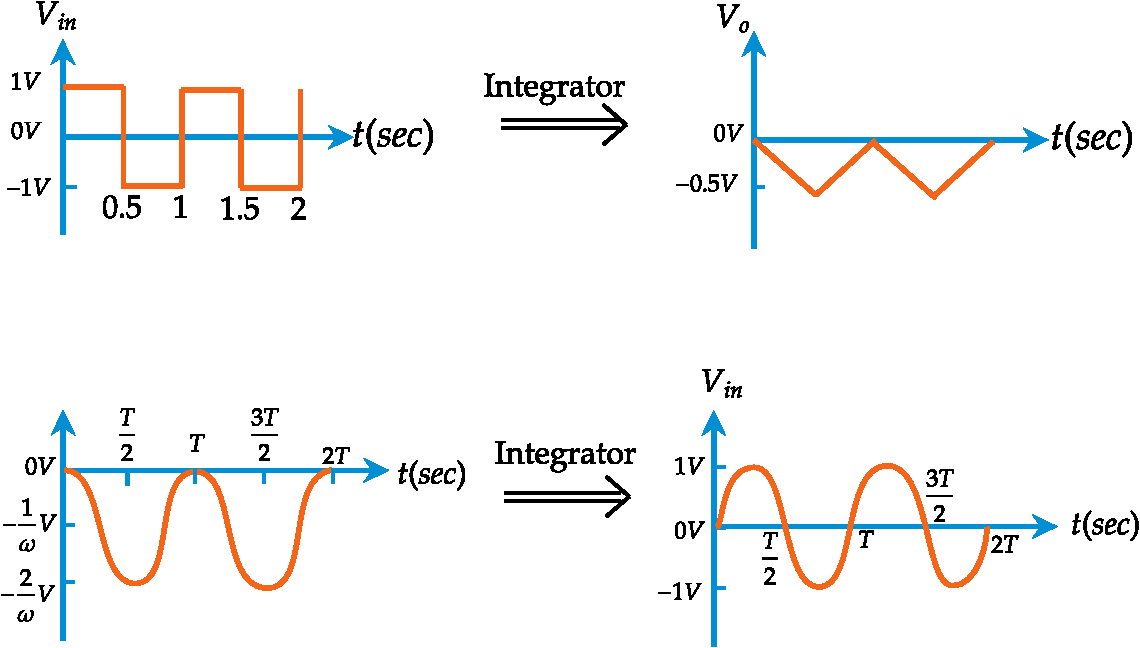
\includegraphics[height=7.5cm,width=10cm]{diagram-20211126(1)-crop}
   	\caption{}
   	\label{}
   \end{figure}
   \subsubsection{Frequency Response of an Integrator}
   \begin{figure}[H]
   	\centering
   	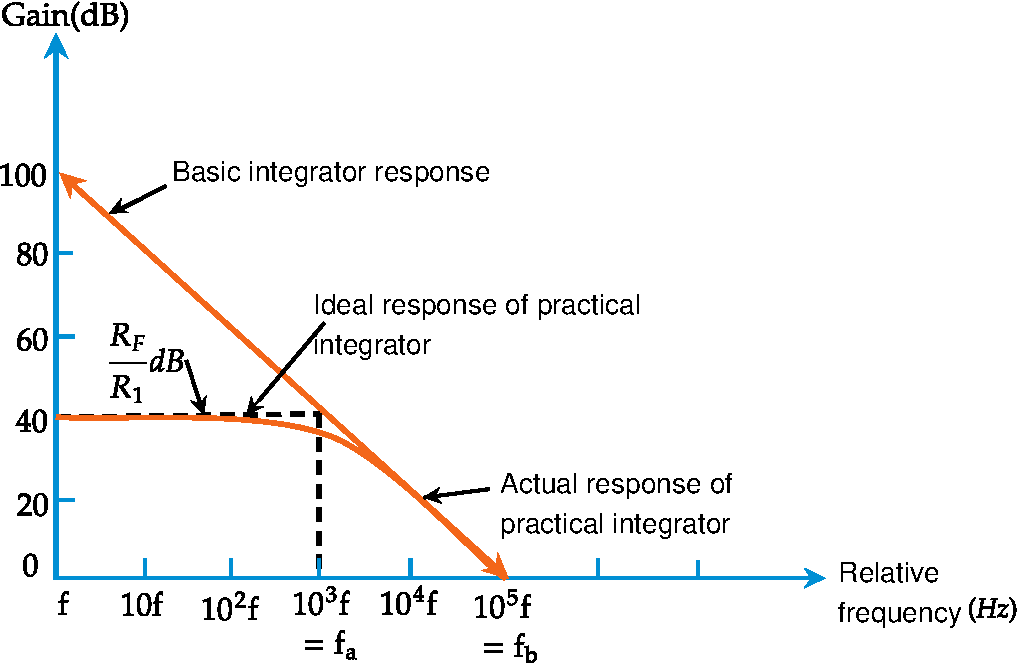
\includegraphics[height=6.5cm,width=10cm]{diagram-20211126(3)-crop}
   	\caption{Frequency Response of an Integrator}
   	\label{Frequency Response of an Integrator}
   \end{figure}
   The frequency response of an integrator is shown in the figure.	\ref{Frequency Response of an Integrator} . $f_b$ is the frequency at which the gain is $0dB$ is given by ,
   \begin{equation}
   f_b=\frac{1}{2 \pi R_1C_F}
   \end{equation}
   But this integrator is not stable which means that the gain is not stable for acertain range of input frequencies.Aslo the gain is  rolled off at low frequencies which means that rate of gain is decreasing at low frequencies.\\
   Both the stability and low frequency roll off problem can be corrected by the addition of a $R_f$ as shown in the practical integrator.\\
   The frequency response of the practical integrator is also shown in the figure.In this figure f is some relative operating frequency , for frequencies f to $f_a$ the gain $\frac{R_F}{R_1}$ is constant.However after $f_a$ the gain decreases at a rate of 20 dB/decade.In other words between $f_a$ and $f_b$ the circuit act as an integrator. The gain limiting frequency $f_a$ is given by ,
   $$f_a=\frac{1}{2 \pi R_F C_F}$$
   \begin{figure}[H]
   	\centering
   	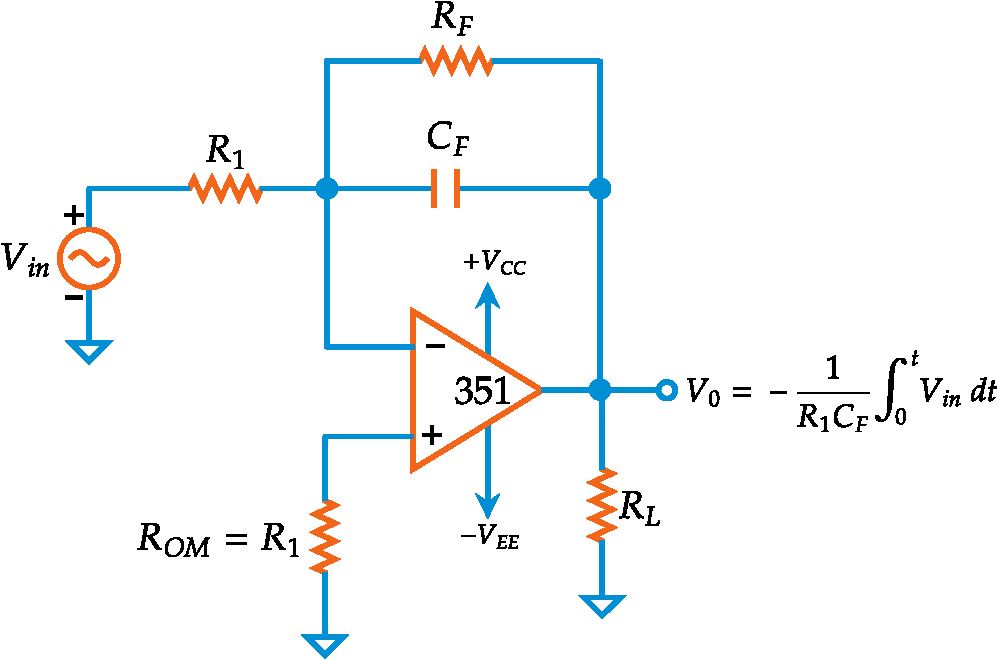
\includegraphics[height=6.5cm,width=10cm]{diagram-20211126(2)-crop}
   	\caption{Practical integrator}
   	\label{}
   \end{figure}
   \subsection{The Differentiator}
   The differentiator or differentiation amplifier circuit performs the mathematical operation of differentiation. That is, the output waveform is the derivative of the input waveform. The differentiator may be constructed from a basic inverting amplifier if an input resistor $R_{1}$ is replaced by a capacitor $C_{1}$.
   \begin{figure}[H]
   	\centering
   	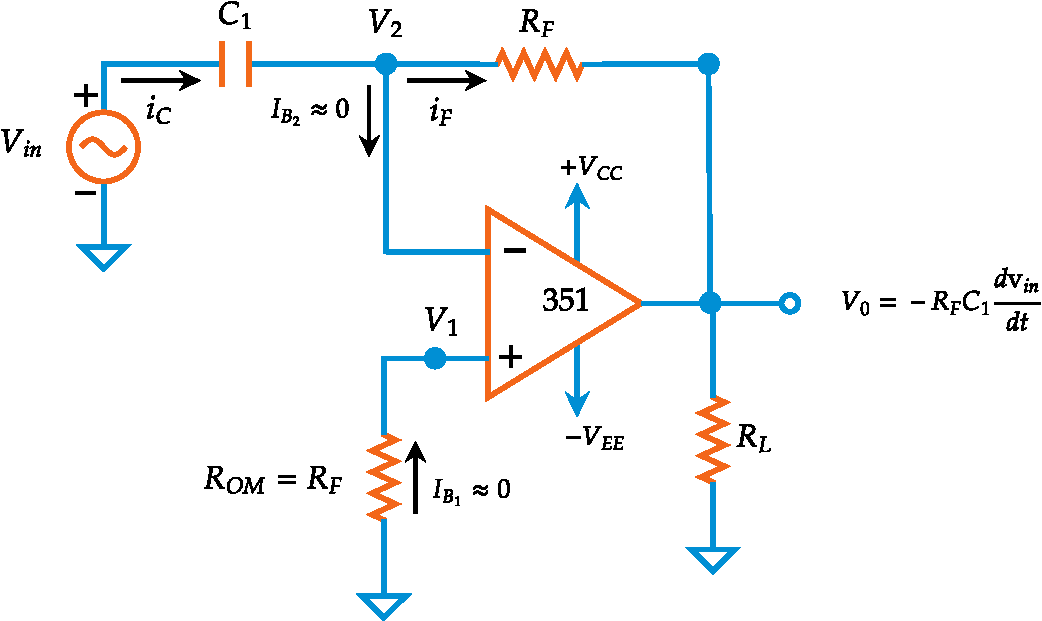
\includegraphics[height=6cm,width=10cm]{diagram-20211127(1)-crop}
   	\caption{}
   	\label{}
   \end{figure}
   
   The expression for the output voltage can be obtained from Kirchhoff's current equation written at node $V_{2}$ as follows:
   
   \begin{align}
   i_{C}&=I_{B}+i_{F}\\
   \text{Since $I_{B} \cong 0$, } \
   i_{C} &=i_{F} \\
   C_{1} \frac{d}{d t}\left(V_{\mathrm{in}}-V_{2}\right) &=\frac{V_{2}-V_{o}}{R_{F}}\\
   \intertext{But $V_{1}=V_{2} \cong 0 \mathrm{~V}$, because $A$ is very large. Therefore, }
   C_{1} \frac{d V_{\mathrm{in}}}{d t}&=-\frac{V_{o}}{R_{F}}\\
   \text{Or }\
   V_{o}&=-R_{F} C_{1} \frac{d V_{\text {in }}}{d t}
   \end{align}
   Thus the output $V_{o}$ is equal to $R_{F} C_{1}$ times the negative instantaneous rate of change of the input voltage $V_{\text {in }}$ with time. Since the differentiator performs the reverse of the integrator's function, a cosine wave input will produce a sine wave output, ol a triangular input will produce a square wave output.
   \begin{figure}[H]
   	\centering
   	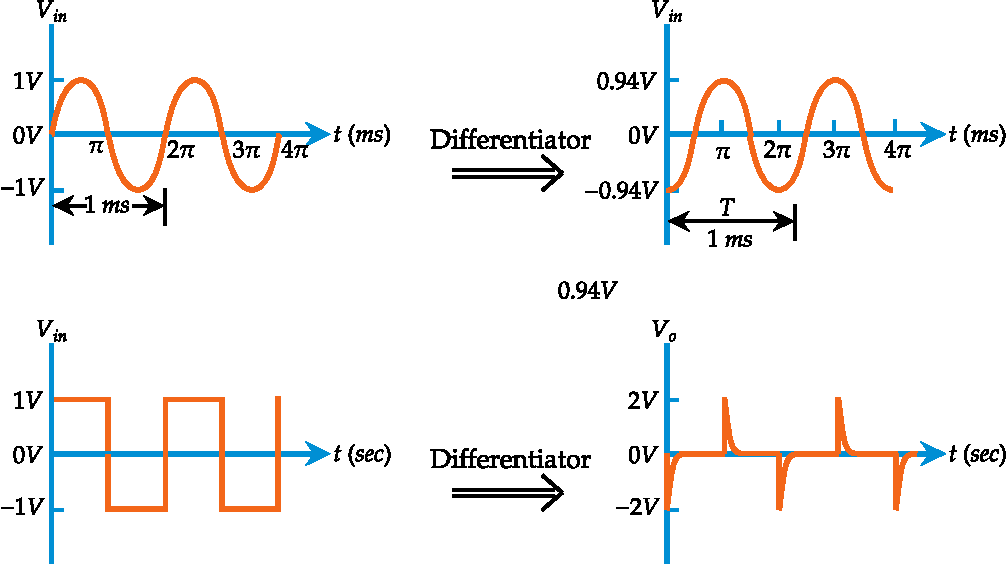
\includegraphics[height=6.5cm,width=10cm]{diagram-20211127(3)-crop}
   	\caption{}
   	\label{}
   \end{figure} 
   \subsubsection{Frequency Response of a Differentiator}
   \begin{figure}[H]
   	\centering
   	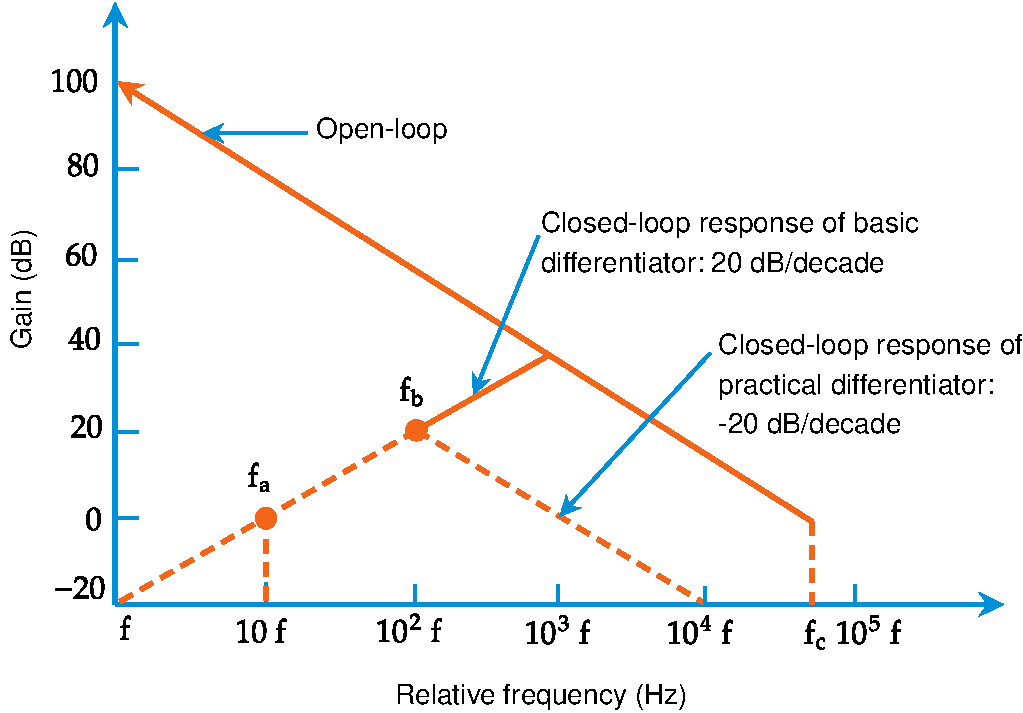
\includegraphics[height=7.8cm,width=10cm]{diagram-20211126(4)-crop}
   	\caption{Frequency Response of a Differentiator}
   	\label{Frequency  Differentiator}
   \end{figure}
   The frequency response of a basic differentiator is shown in the figure.\ref{Frequency  Differentiator}
   In this figure.\ref{Frequency  Differentiator} , $f_a$ is the frequency at which the gain is the $0dB$ and is given by,
   \begin{equation}
   f_a=\frac{1}{2 \pi R_FC_1}
   \end{equation}
   And $f_c$ is the unit gain band width of the op-amp and f is some relative opertaing frequency.\\
   \paragraph{Drawback of this differentiator}
   \begin{note}
   	\begin{itemize}
   		\item The gain of the circuit $\frac{R_F}{X_{CI}}$ increase with increase in frequency at the rate of 20 dB/decade.This makes the circuit very unstable.
   		\item The input impedance $X_{C1}$ secreases with increase in frequency.which makes the circuit very susceptible to high frequency noise.When amplified this noise can be completely override the differentiated output signal.
   	\end{itemize}
   \end{note}
   Both the stability and the high-frequency noise problems can be corrected by the addition of two components: $R_{1}$ and $C_{F}$, as shown in Figure bellow. This circuit is a practical differentiator. From frequency $f$ to $f_{b}$, the gain increases at $20 \mathrm{~dB} / \mathrm{decade}$. However, after $f_{b}$ the gain decreases at $20 \mathrm{~dB} /$ decade. This 40 . $\mathrm{dB} /$ decade change in gain is caused by the $R_{1} C_{1}$ and $R_{F} C_{F}$ combinations. The gain. limiting frequency $f_{b}$ is given by,
   $$f_{b}=\frac{1}{2 \pi R_{1} C_{1}}$$
   Where  $R_{1} C_{1}=R_{F} C_{F}$\\
   Thus $R_{1} C_{1}$ and $R_{F} C_{F}$ help to reduce significantly the effect of high-frequency input, amplifier noise, and offsets. Above all, $R_{1} C_{1}$ and $R_{F} C_{F}$ make the circuit more stable by preventing the increase in gain with frequency. Generally, the value of $f_{b}$ and in turn $R_{1} C_{1}$ and $R_{F} C_{F}$ values should be selected such that
   $$
   f_{a}<f_{b}<f_{c}
   $$
   $$\begin{aligned}
   &f_{a}=\frac{1}{2 \pi R_{F} C_{1}} \\
   &f_{b}=\frac{1}{2 \pi R_{1} C_{1}}=\frac{1}{2 \pi R_{F} C_{F}} \\
   &f_{c}=\text { unity gain-bandwidth }
   \end{aligned}$$
   \begin{figure}[H]
   	\centering
   	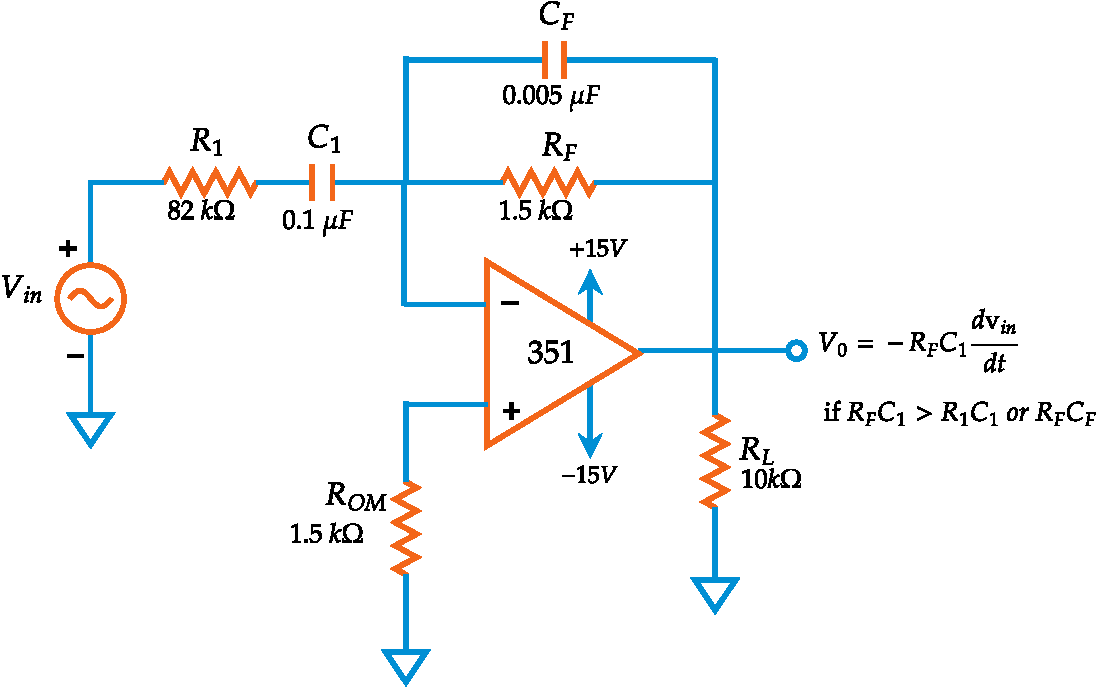
\includegraphics[height=7cm,width=12cm]{diagram-20211126(5)-crop}
   	\caption{}
   	\label{}
   \end{figure}
   \newpage
   \begin{abox}
   Practice Set- 1
   \end{abox}
\begin{enumerate}
	\item A time varying signal $V_{i n}$ is fed to an op-amp circuit with output signal $V_{o}$ as shown in the figure below.\\
	\begin{figure}[H]
		\centering
		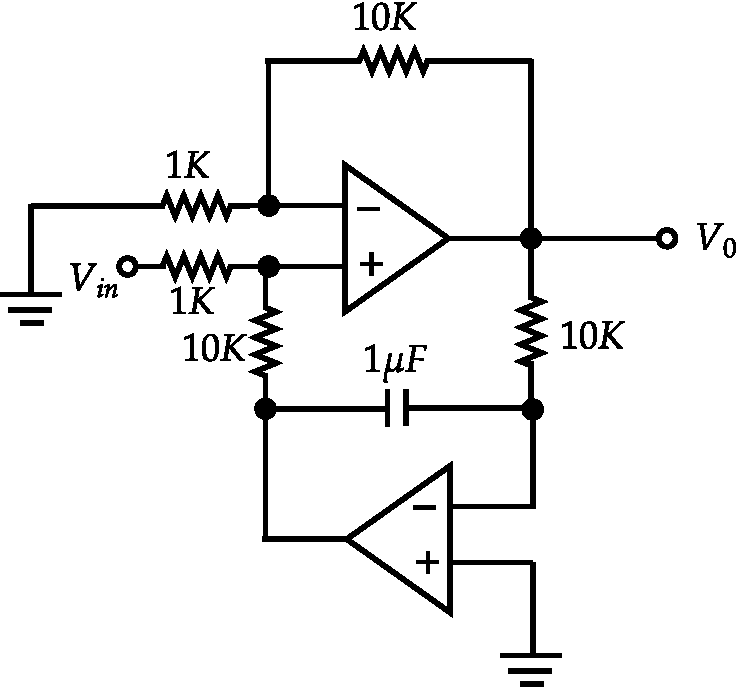
\includegraphics[height=6cm,width=6.5cm]{diagram-20211018(1)-crop}
	\end{figure}
	The circuit implements a
	{\exyear{NET/JRF(JUNE-2011)}}
\begin{tasks}(1)
\task[\textbf{A.}] High pass filter with cutoff frequency $16 \mathrm{~Hz}$
\task[\textbf{B.}] High pass filter with cutoff frequency $100 \mathrm{~Hz}$
\task[\textbf{C.}] Low pass filter with cutoff frequency $16 \mathrm{~Hz}$
\task[\textbf{D.}] Low pass filter with cutoff frequency $100 \mathrm{~Hz}$
\end{tasks}
	\item In the operational amplifier circuit below, the voltage at point $A$ is
{	\exyear{NET/JRF(DEC-2011)}}
\begin{figure}[H]
\centering
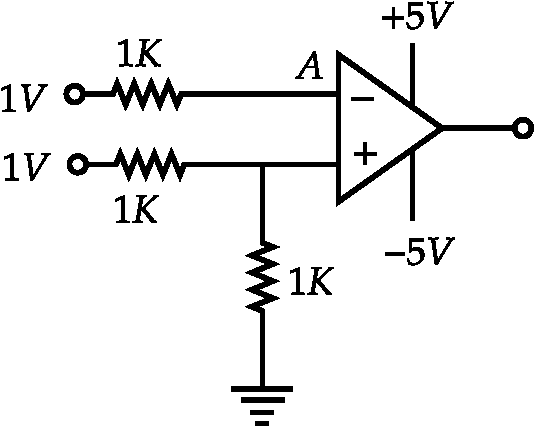
\includegraphics[height=4cm,width=5.5cm]{diagram-20211018(2)-crop}
\end{figure}
\begin{tasks}(4)
\task[\textbf{A.}] $1.0 \mathrm{~V}$
\task[\textbf{B.}] $0.5 \mathrm{~V}$
\task[\textbf{C.}] $0 \mathrm{~V}$
\task[\textbf{D.}] $-5.0 V$
\end{tasks}
	\item In the op-amp circuit shown in the figure below, the input voltage is $1 \mathrm{~V}$. The value of the output $\mathrm{V}_{0}$ is
	{\exyear{NET/JRF(JUNE-2012)}}
\begin{figure}[H]
\centering
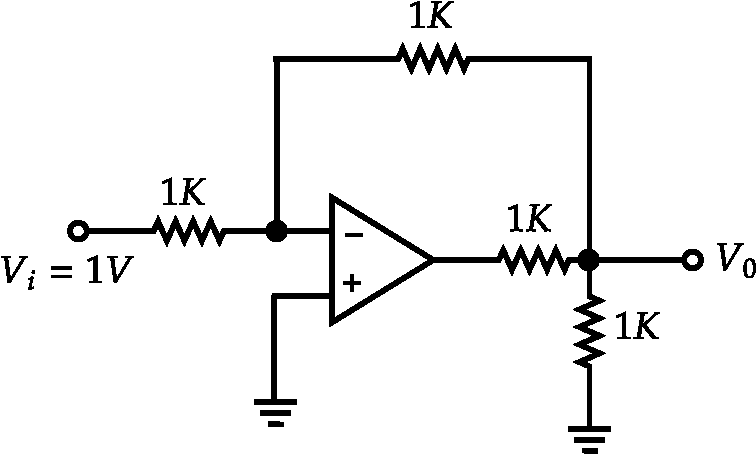
\includegraphics[height=3.5cm,width=6cm]{e-08}
\end{figure}
\begin{tasks}(4)
\task[\textbf{A.}] $-0.33 \mathrm{~V}$
\task[\textbf{B.}] $-0.50 \mathrm{~V}$
\task[\textbf{C.}] $-1.00 \mathrm{~V}$
\task[\textbf{D.}] $-0.25 \mathrm{~V}$
\end{tasks}
	\item In the op-amp circuit shown in the figure, $V_{i}$ is a sinusoidal input signal of frequency 10 $\mathrm{Hz}$ and $V_{0}$ is the output signal. The magnitude of the gain and the phase shift, respectively, close to the values
{	\exyear{NET/JRF(DEC-2012)}}
\begin{tasks}(1)
	\task[\textbf{A.}] $5 \sqrt{2}$ and $\pi / 2$
	\task[\textbf{B.}] $5 \sqrt{2}$ and $-\pi / 2$
	\task[\textbf{C.}] 10 and zero
	\task[\textbf{D.}] 10 and $\pi$
\end{tasks}
\begin{minipage}{0.45\textwidth}
\begin{figure}[H]
	\centering
	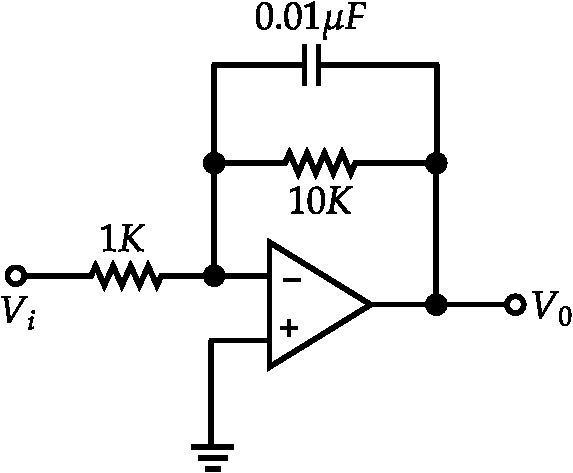
\includegraphics[height=4cm,width=5cm]{e-13}
\end{figure}
\end{minipage}
	\item Consider the op-amp circuit shown in the figure.
	If the input is a sinusoidal wave $V_{i}=5 \sin (1000 t)$, then the amplitude of the output $V_{0}$ is
{	\exyear{NET/JRF(DEC-2013)}}
\begin{figure}[H]
\centering
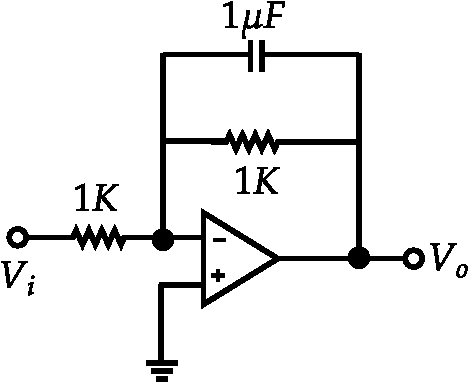
\includegraphics[height=3.5cm,width=4.5cm]{e-21}
\end{figure}
\begin{tasks}(4)
\task[\textbf{A.}] $\frac{5}{2}$
\task[\textbf{B.}]  5
\task[\textbf{C.}] $\frac{5 \sqrt{2}}{2}$
\task[\textbf{D.}] $5 \sqrt{2}$
\end{tasks}
	\item The inner shield of a triaxial conductor is driven by an (ideal) op-amp follower circuit as shown. The effective capacitance between the signal-carrying conductor and ground is
{	\exyear{NET/JRF(JUNE-2014)}}
\begin{figure}[H]
\centering
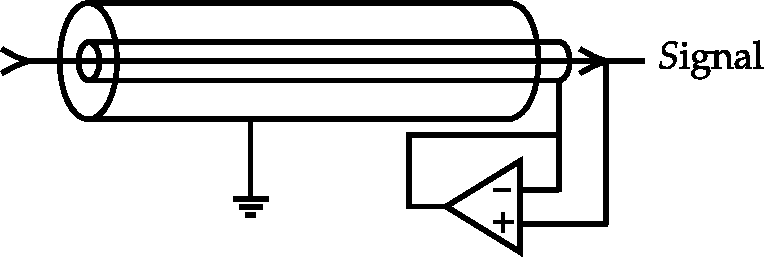
\includegraphics[height=2.5cm,width=7cm]{e-26}
\end{figure}
\begin{tasks}(4)
\task[\textbf{A.}]  Unaffected
\task[\textbf{B.}] Doubled
\task[\textbf{C.}] Halved
\task[\textbf{D.}] Made zero
\end{tasks}
	\item Consider the amplifier circuit comprising of the two op-amps $A_{1}$ and $A_{2}$ as shown in the in the figure. \\
	\begin{figure}[H]
		\centering
		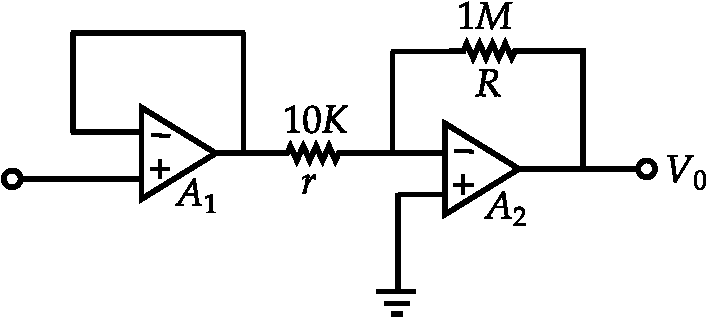
\includegraphics[height=3cm,width=7cm]{e-30}
	\end{figure}
	If the input ac signal source has an impedance of $50 k \Omega$, which of the following statements is true?
{	\exyear{NET/JRF(DEC-2014)}}
\begin{tasks}(1)
\task[\textbf{A.}] $A_{1}$ is required in the circuit because the source impedance is much greater than $r$
\task[\textbf{B.}] $A_{1}$ is required in the circuit because the source impedance is much less than $R$
\task[\textbf{C.}] $A_{1}$ can be eliminated from the circuit without affecting the overall gain
\task[\textbf{D.}] $A_{1}$ is required in the circuit if the output has to follow the phase of the input signal
\end{tasks}
	\item Consider a Low Pass (LP) and a High Pass (HP) filter with cut-off frequencies $f_{L P}$ and $f_{H P}$, respectively, connected in series or in parallel configurations as shown in the Figures A and B below.\\
	\begin{figure}[H]
		\centering
		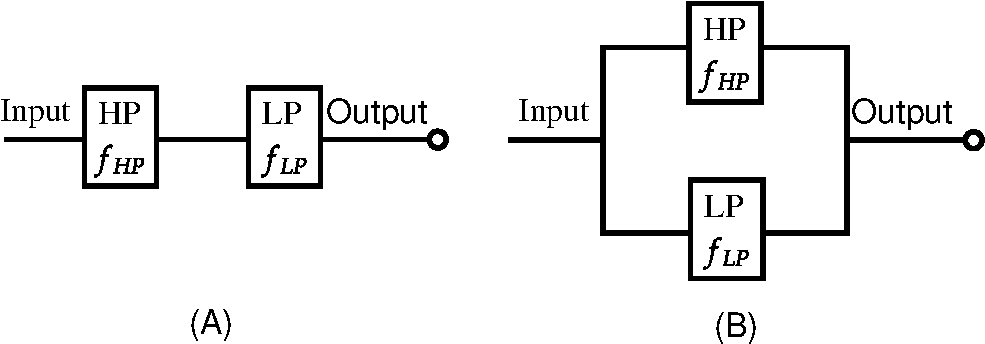
\includegraphics[height=4cm,width=10cm]{e-33}
	\end{figure}
	Which of the following statements is correct?
{	\exyear{NET/JRF(DEC-2014)}}
\begin{tasks}(1)
\task[\textbf{A.}] For $f_{H P}<f_{L P}$, A acts as a Band Pass filter and B acts as a band Reject filter
\task[\textbf{B.}] For $f_{H P}>f_{L P}$, A stops the signal from passing through and B passes the signal without filtering
\task[\textbf{C.}] For $f_{H P}<f_{L P}$, A acts as a Band Pass filter and B passes the signal without filtering
\task[\textbf{D.}] For $f_{H P}>f_{L P}$, A passes the signal without filtering and B acts as a Band Reject filter
\end{tasks}
	\item In the circuit given below, the thermistor has a resistance $3 k \Omega$ at $25^{0} C$. Its resistance decreases by $150 \Omega$ per ${ }^{0} C$ upon heating. The output voltage of the circuit at $30^{\circ} \mathrm{C}$ is
{	\exyear{NET/JRF(JUNE-2015)}}
\begin{figure}[H]
\centering
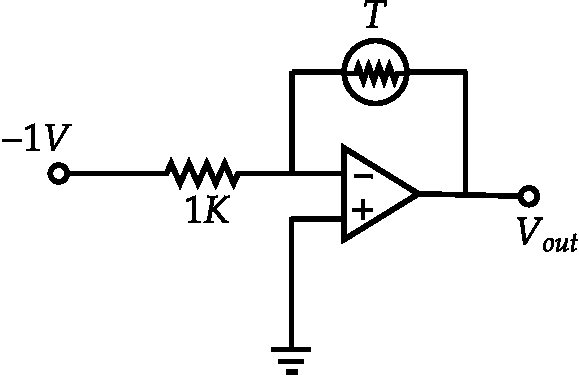
\includegraphics[height=3.5cm,width=5.5cm]{e-38}
\end{figure}
\begin{tasks}(4)
\task[\textbf{A.}] $-3.75 \mathrm{~V}$
\task[\textbf{B.}] $-2.25 \mathrm{~V}$
\task[\textbf{C.}] $2.25 \mathrm{~V}$
\task[\textbf{D.}] $3.75 \mathrm{~V}$
\end{tasks}
	\item If the parameters $y$ and $x$ are related by $y=\log (x)$, then the circuit that can be used to produce an output voltage $V_{0}$ varying linearly with $x$ is
	{\exyear{NET/JRF(DEC-2015)}}
\begin{tasks}(2)
\task[\textbf{A.}] \begin{figure}[H]
	\centering
	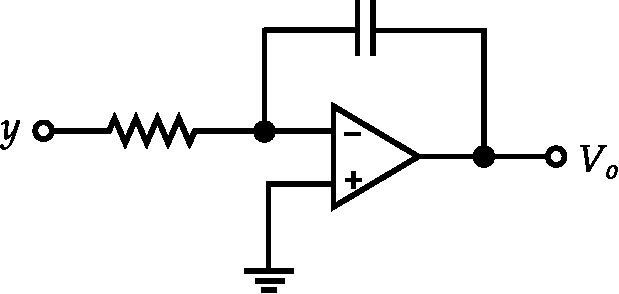
\includegraphics[height=3cm,width=5.5cm]{e40a}
\end{figure}
\task[\textbf{B.}] \begin{figure}[H]
	\centering
	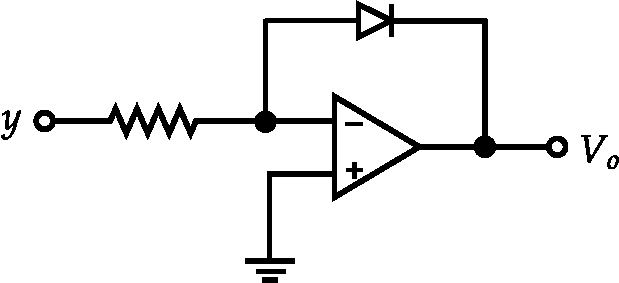
\includegraphics[height=3cm,width=5.5cm]{e40b}
\end{figure}
\task[\textbf{C.}] \begin{figure}[H]
	\centering
	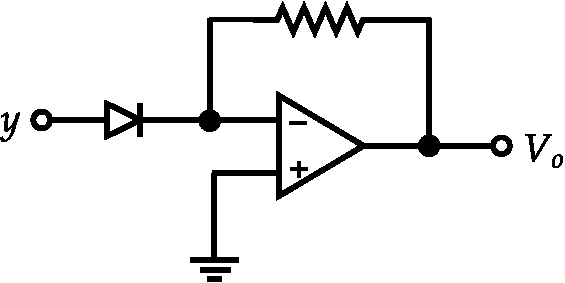
\includegraphics[height=3cm,width=5.5cm]{e40c}
\end{figure}
\task[\textbf{D.}] \begin{figure}[H]
	\centering
	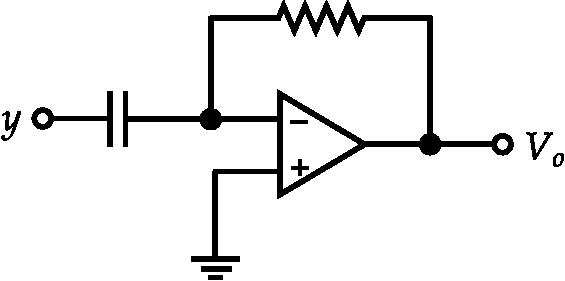
\includegraphics[height=3cm,width=5.5cm]{e40d}
\end{figure}
\end{tasks}
	\item A sinusoidal signal of peak to peak amplitude $1 V$ and unknown time period is input to the following circuit for 5 second's duration. If the counter measures a value $(3 E 8)_{H}$ in hexadecimal, then the time period of the input signal is
{	\exyear{NET/JRF(DEC-2015)}}
\begin{figure}[H]
\centering
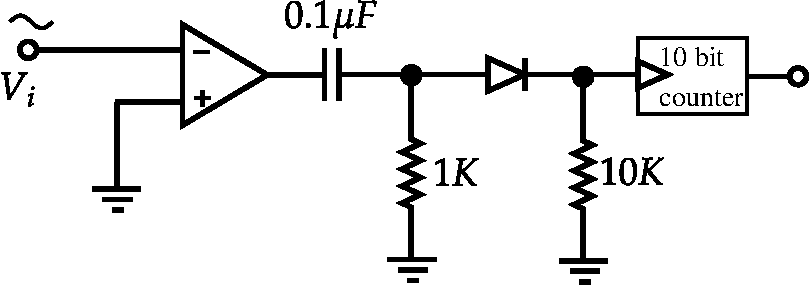
\includegraphics[height=3cm,width=8cm]{e42}
\end{figure}
\begin{tasks}(4)
\task[\textbf{A.}] $2.5 \mathrm{~ms}$
\task[\textbf{B.}] $4 \mathrm{~ms}$
\task[\textbf{C.}]  $10 \mathrm{~ms}$
\task[\textbf{D.}] $5 \mathrm{~ms}$
\end{tasks}
	\item Given the input voltage $V_{i}$, which of the following waveforms correctly represents the output voltage $V_{0}$ in the circuit shown below?
{	\exyear{NET/JRF(JUNE-2016)}}
\begin{figure}[H]
\centering
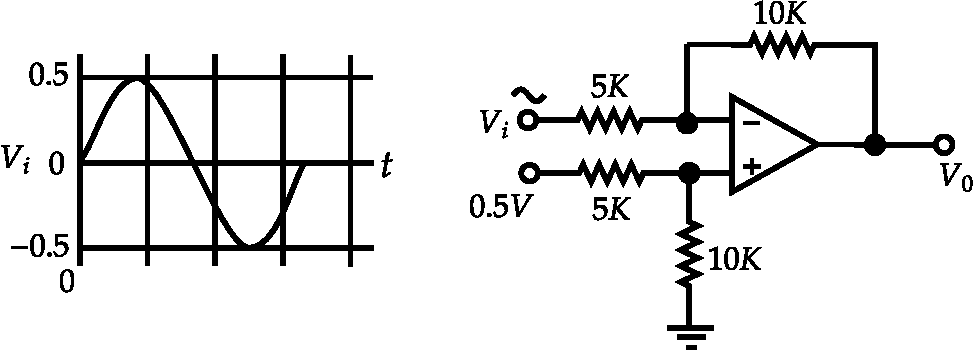
\includegraphics[height=3.5cm,width=10cm]{diagram-20211020(13)-crop}
\end{figure}
\begin{tasks}(2)
\task[\textbf{A.}] \begin{figure}[H]
	\centering
	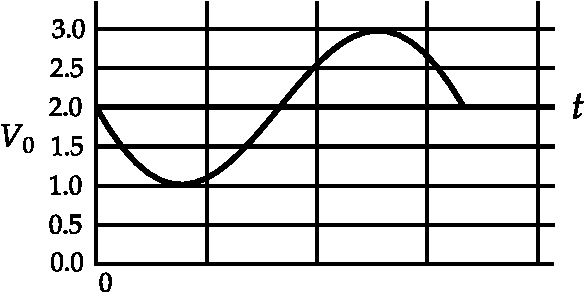
\includegraphics[height=3cm,width=5.5cm]{diagram-20211020(14)-crop}
\end{figure}
\task[\textbf{B.}] \begin{figure}[H]
	\centering
	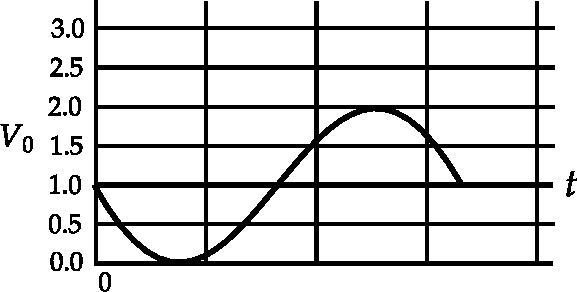
\includegraphics[height=3cm,width=5.5cm]{diagram-20211020(15)-crop}
\end{figure}
\task[\textbf{C.}] \begin{figure}[H]
	\centering
	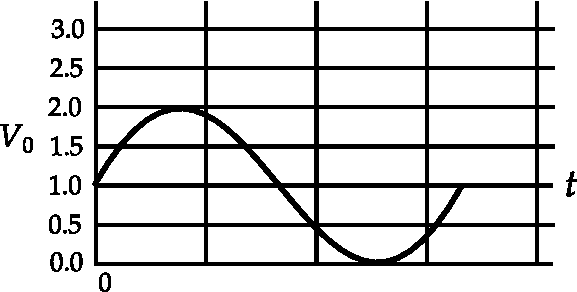
\includegraphics[height=3cm,width=5.5cm]{diagram-20211020(16)-crop}
\end{figure}
\task[\textbf{D.}] \begin{figure}[H]
	\centering
	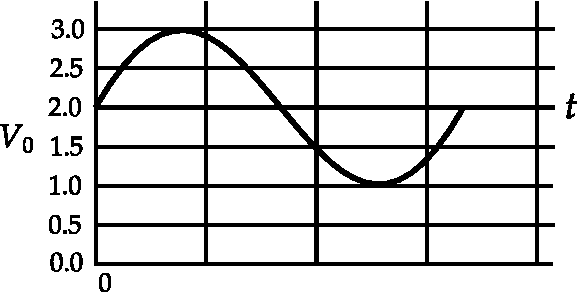
\includegraphics[height=3cm,width=5.5cm]{diagram-20211020(17)-crop}
\end{figure}
\end{tasks}
	\item  In the circuit below, the input voltage $V_{i}$ is $2 V, V_{c c}=16 \mathrm{~V}, R_{2}=2 \mathrm{k} \Omega$ and $R_{L}=10 \mathrm{k} \Omega$\\
	\begin{figure}[H]
		\centering
		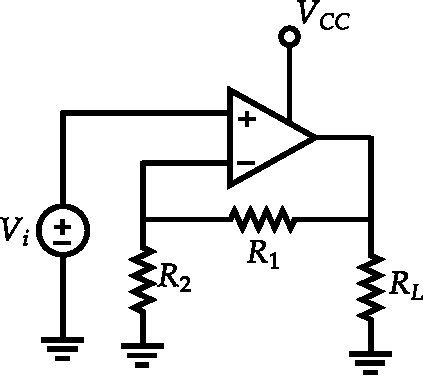
\includegraphics[height=3.5cm,width=4.5cm]{e50}
	\end{figure}
	The value of $R_{1}$ required to deliver $10 \mathrm{~mW}$ of power across $R_{L}$ is
	{\exyear{NET/JRF(DEC-2016)}}
\begin{tasks}(4)
\task[\textbf{A.}] $12 k \Omega$
\task[\textbf{B.}] $4 k \Omega$
\task[\textbf{C.}]  $8 \mathrm{k} \Omega$
\task[\textbf{D.}]  $14 k \Omega$
\end{tasks}                
	\item The gain of the circuit given below is $-\frac{1}{\omega R C}$.\\
	\begin{figure}[H]
		\centering
		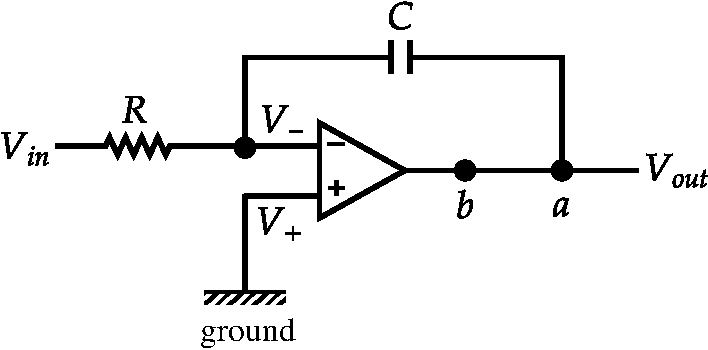
\includegraphics[height=3.5cm,width=6.5cm]{e54}
	\end{figure}
	The modification in the circuit required to introduce a dc feedback is to add a resistor
	{\exyear{NET/JRF(JUNE-2017)}}
\begin{tasks}(1)
\task[\textbf{A.}] Between $a$ and $b$
\task[\textbf{B.}]  Between positive terminal of the op-amp and ground
\task[\textbf{C.}] In series with $C$
\task[\textbf{D.}] Parallel to $C$
\end{tasks}
	\item In the following operational amplifier circuit $C_{i n}=10 n F, R_{i n}=20 k \Omega, R_{F}=200 k \Omega$ and $C_{F}=100 \mathrm{pF}$\\
	\begin{figure}[H]
		\centering
		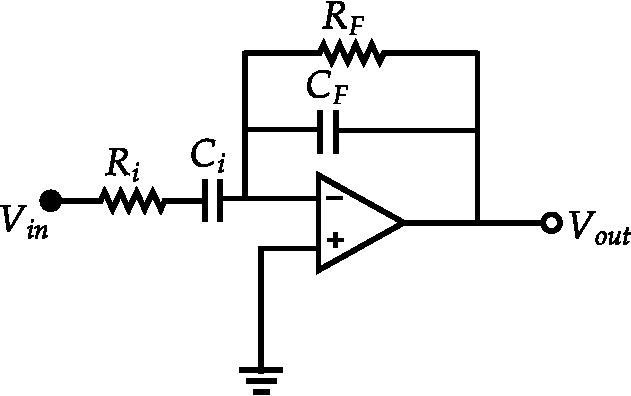
\includegraphics[height=3.5cm,width=6cm]{e60}
	\end{figure}
	The magnitude of the gain at a input signal frequency of $16 \mathrm{kHz}$ is
	{\exyear{NET/JRF(JUNE-2017)}}
\begin{tasks}(4)
\task[\textbf{A.}] 67
\task[\textbf{B.}] $0.15$
\task[\textbf{C.}] $0.3$
\task[\textbf{D.}] $3.5$
\end{tasks}
	\item Two signals $A_{1} \sin (\omega t)$ and $A_{2} \cos (\omega t)$ are fed into the input and the reference channels, respectively, of a lock-in amplifier. The amplitude of each signal is $1 V$. The time constant of the lock-in amplifier is such that any signal of frequency larger than $\omega$ is filtered out. The output of the lock-in amplifier is
	{\exyear{NET/JRF(JUNE-2018)}}
\begin{tasks}(4)
\task[\textbf{A.}]  $2 V$
\task[\textbf{B.}] $1 \mathrm{~V}$
\task[\textbf{C.}] $0.5 \mathrm{~V}$
\task[\textbf{D.}] $0 V$
\end{tasks}
	\item The input $V_i$ to the following circuit is a square wave as shown in the following figure\\
	\begin{figure}[H]
		\centering
		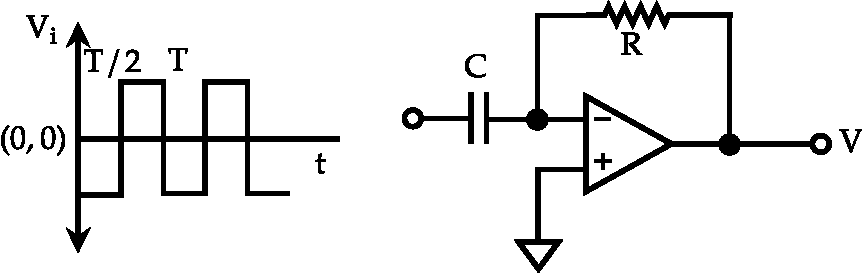
\includegraphics[height=3cm,width=8cm]{e73}
	\end{figure}
	Which of the waveforms $V_0$ best describes the output?
{	\exyear{NET/JRF(JUNE-2018)}}
\begin{tasks}(2)
\task[\textbf{A.}] \begin{figure}[H]
	\centering
	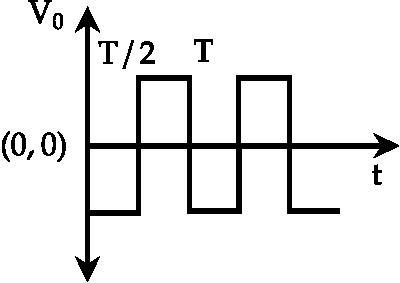
\includegraphics[height=3cm,width=5cm]{e73a}
\end{figure}
\task[\textbf{B.}] \begin{figure}[H]
	\centering
	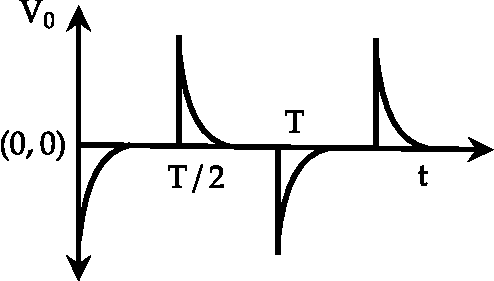
\includegraphics[height=3cm,width=5cm]{e73b}
\end{figure}
\task[\textbf{C.}] \begin{figure}[H]
	\centering
	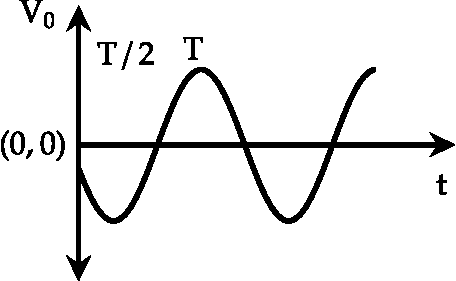
\includegraphics[height=3cm,width=5cm]{e73c}
\end{figure}
\task[\textbf{D.}] \begin{figure}[H]
	\centering
	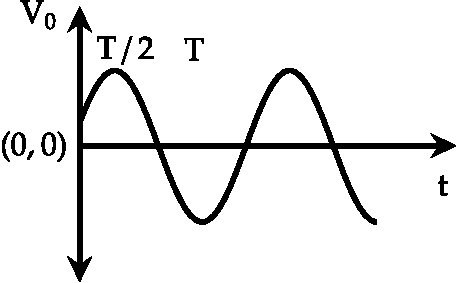
\includegraphics[height=3cm,width=5cm]{e73d}
\end{figure}
\end{tasks}
	\item The input $V_ i$ to the following circuit is a square wave as shown in the following figure.\\
	\begin{figure}[H]
		\centering
		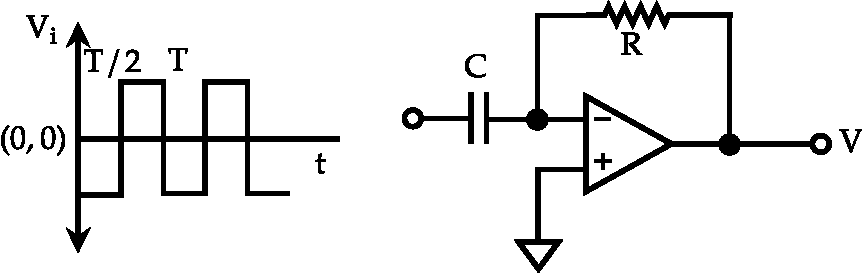
\includegraphics[height=2.5cm,width=8cm]{e73}
	\end{figure}
	which of the waveforms best describes the output?
{	\exyear{NET/JRF(DEC-2018)}}
\begin{tasks}(2)
\task[\textbf{A.}] \begin{figure}[H]
	\centering
	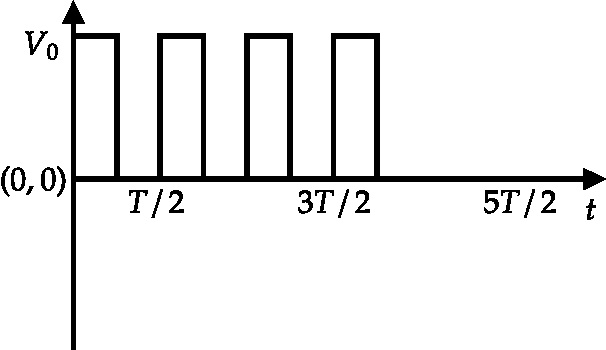
\includegraphics[height=3cm,width=5cm]{e74a}
\end{figure}
\task[\textbf{B.}] \begin{figure}[H]
	\centering
	\includegraphics[height=3cm,width=5cm]{e74b}
\end{figure}
\task[\textbf{C.}] \begin{figure}[H]
	\centering
	\includegraphics[height=3cm,width=5cm]{e74c}
\end{figure}
\task[\textbf{D.}]\begin{figure}[H]
	\centering
	\includegraphics[height=3cm,width=5cm]{e74d}
\end{figure}
\end{tasks}
	\item A circuit constructed using op-amp, resistor $R_{1}=1 \mathrm{k} \Omega$ and capacitors $C_{1}=1 \mu \mathrm{F}$ and $C_{2}=0.1 \mu F$ is shown in the figure below.\\
	\begin{figure}[H]
		\centering
		\includegraphics[height=4cm,width=5cm]{diagram-20211029(7)-crop}
	\end{figure}
	This circuit will act as a
{	\exyear{NET/JRF(JUNE-2019)}}
\begin{tasks}(2)
\task[\textbf{A.}] High pass filter
\task[\textbf{B.}] Low pass filter
\task[\textbf{C.}] Band pass filter
\task[\textbf{D.}] Band reject filter
\end{tasks}
	\item In the circuit diagram of a band pass filter shown below, $R=10 \mathrm{k} \Omega$.\\
	\begin{figure}[H]
		\centering
		\includegraphics[height=3.5cm,width=8cm]{diagram-20211029(10)-crop}
	\end{figure}
	In order to get a lower cut-off frequency of $150 \mathrm{~Hz}$ and an upper cut-off frequency of $10 \mathrm{kHz}$, the appropriate values of $C_{1}$ and $C_{2}$ respectively are
{	\exyear{NET/JRF(DEC-2019)}}
\begin{tasks}(2)
\task[\textbf{A.}]  $0.1 \mu F$ and $1.5 n F$
\task[\textbf{B.}] $0.3 \mu \mathrm{F}$ and $5.0 \mathrm{nF}$
\task[\textbf{C.}] $1.5 n F$ and $0.1 \mu F$
\task[\textbf{D.}]  $5.0 \mathrm{nF}$ and $0.3 \mu \mathrm{F}$
\end{tasks}
	\item The $I-V$ characteristics of the diode $D$ in the circuit below is given by
	$$
	I=I_{s}\left(e^{\frac{q V}{k_{\mathrm{B}} T}}-1\right)
	$$
	where $I_{s}$ is the reverse saturation current, $V$ is the voltage across the diode and $T$ is the absolute temperature.\\
	\begin{figure}[H]
		\centering
		\includegraphics[height=3.5cm,width=6cm]{diagram-20211030(4)-crop}
		\caption{}
		\label{}
	\end{figure}
	If the input voltage is $V_{\text {in }}$, then the output voltage $V_{\text {out }}$ is
{	\exyear{NET/JRF(JUNE-2020)}}
\begin{tasks}(2)
\task[\textbf{A.}] (a) $I_{s} R \ln \left(\frac{q V_{\text {in }}}{k_{B} T}+1\right)$
\task[\textbf{B.}] $\frac{1}{q} k_{B} T \ln \left(\frac{q\left(V_{\text {in }}+I_{s} R\right)}{k_{B} T}\right)$
\task[\textbf{C.}]  $\frac{1}{q} k_{B} T \ln \left(\frac{V_{\text {in }}}{I_{s} R}+1\right)$
\task[\textbf{D.}]  $-\frac{1}{q} k_{B} T \ln \left(\frac{V_{\text {in }}}{I_{s} R}+1\right)$
\end{tasks}
	\item In the circuit shown below, the gain of the op-amp in the middle of its bandwidth is $10^{5}$. A sinusoidal voltage with angular frequency $\omega=100 \mathrm{rad} / \mathrm{s}$ is applied to the input of the op-amp.\\
	\begin{figure}[H]
		\centering
		\includegraphics[height=4cm,width=7cm]{diagram-20211030(5)-crop}
		\caption{}
		\label{}
	\end{figure}
	The phase difference between the input and the output voltage is
{	\exyear{NET/JRF(JUNE-2020)}}
\begin{tasks}(4)
\task[\textbf{A.}]  $5 \pi / 4$
\task[\textbf{B.}] $3 \pi / 4$
\task[\textbf{C.}] $\pi / 2$
\task[\textbf{D.}] $\pi$
\end{tasks}
\end{enumerate}
 \colorlet{ocre1}{ocre!70!}
\colorlet{ocrel}{ocre!30!}
\setlength\arrayrulewidth{1pt}
\begin{table}[H]
	\centering
	\arrayrulecolor{ocre}
	\begin{tabular}{|p{1.5cm}|p{1.5cm}||p{1.5cm}|p{1.5cm}|}
		\hline
		\multicolumn{4}{|c|}{\textbf{Answer key}}\\\hline\hline
		\rowcolor{ocrel}Q.No.&Answer&Q.No.&Answer\\\hline
		1&\textbf{C} &2&\textbf{B}\\\hline 
		3&\textbf{B} &4&\textbf{D} \\\hline
		5&\textbf{C} &6&\textbf{A} \\\hline
		7&\textbf{A}&8&\textbf{C}\\\hline
		9&\textbf{C}&10&\textbf{C}\\\hline
		11&\textbf{D} &12&\textbf{B}\\\hline
		13&\textbf{C}&14&\textbf{D}\\\hline
		15&\textbf{D}&16&\textbf{D} \\\hline
		17&\textbf{B}&18&\textbf{C}\\\hline
		19&\textbf{A}&20&\textbf{A}\\\hline
		21&\textbf{C} &22&\textbf{A}\\\hline
		
	\end{tabular}
\end{table}
 \newpage
 \begin{abox}
 	Practice Set- 2
 \end{abox}
 \begin{enumerate}
 	\item In one of the following circuits, negative feedback does not operate for a negative input. Which one is it? The opamps are running from $\pm 15 \mathrm{~V}$ supplies.
 	{\exyear{GATE 2010}}
 	\begin{tasks}(2)
 		\task[\textbf{A.}] \begin{figure}[H]
 			\centering
 			\includegraphics[height=3.5cm,width=4cm]{diagram-20210912(9)-crop}
 		\end{figure}
 		\task[\textbf{B.}] \begin{figure}[H]
 			\centering
 			\includegraphics[height=3.5cm,width=4cm]{diagram-20210912(10)-crop}
 		\end{figure}
 		\task[\textbf{C.}] \begin{figure}[H]
 			\centering
 			\includegraphics[height=3.5cm,width=4cm]{diagram-20210912(11)-crop}
 		\end{figure}
 		\task[\textbf{D.}] \begin{figure}[H]
 			\centering
 			\includegraphics[height=3.5cm,width=4cm]{diagram-20210912(12)-crop}
 		\end{figure}
 	\end{tasks}
 	\item Consider the following circuit.\\
 	\begin{figure}[H]
 		\centering
 		\includegraphics[height=3.5cm,width=7cm]{diagram-20210913(6)-crop}
 	\end{figure}
 	Which of the following correctly represents the output $V_{\text {out }}$ corresponding to the input $V_{i n} ?$
 	{\exyear{GATE 2011}}
 	\begin{tasks}(2)
 		\task[\textbf{A.}] \begin{figure}[H]
 			\centering
 			\includegraphics[height=6.5cm,width=6cm]{diagram-20210913(2)-crop}
 		\end{figure}
 		\task[\textbf{B.}] \begin{figure}[H]
 			\centering
 			\includegraphics[height=6.5cm,width=6cm]{diagram-20210913(3)-crop}
 		\end{figure}
 		\task[\textbf{C.}]\begin{figure}[H]
 			\centering
 			\includegraphics[height=6.5cm,width=6cm]{diagram-20210913(4)-crop}
 		\end{figure}
 		\task[\textbf{D.}] \begin{figure}[H]
 			\centering
 			\includegraphics[height=6.5cm,width=6cm]{diagram-20210913(5)-crop}
 		\end{figure}
 	\end{tasks}
 	\item If the peak output voltage of a full wave rectifier is $10 \mathrm{~V}$, its d.c. voltage is
 	{	\exyear{GATE 2012}}
 	\begin{tasks}(4)
 		\task[\textbf{A.}] $10.0 \mathrm{~V}$
 		\task[\textbf{B.}] $7.07 \mathrm{~V}$
 		\task[\textbf{C.}] $6.36 \mathrm{~V}$
 		\task[\textbf{D.}] $3.18 \mathrm{~V}$
 	\end{tasks}
 	\item In the following circuit, for the output voltage to be $V_{0}=\left(-V_{1}+V_{2} / 2\right)$ the ratio $R_{1} / R_{2}$ is
 	{	\exyear{GATE 2012}}
 	\begin{figure}[H]
 		\centering
 		\includegraphics[height=5.5cm,width=5.5cm]{diagram-20210913(12)-crop}
 	\end{figure}
 	\begin{tasks}(4)
 		\task[\textbf{A.}] $1 / 2$
 		\task[\textbf{B.}] 1
 		\task[\textbf{C.}] 2
 		\task[\textbf{D.}] 3
 	\end{tasks}
 	\item Consider the following OP-AMP circuit.
 	Which one of the following correctly represents the output $\mathrm{V}_{\text {out }}$ corresponding to the input $\mathrm{V}_{\text {in }}$ ?
 	{	\exyear{GATE 2012}}
 	\begin{figure}[H]
 		\centering
 		\includegraphics[height=4.5cm,width=5.5cm]{diagram-20210913(13)-crop}
 	\end{figure}
 	\begin{tasks}(2)
 		\task[\textbf{A.}] \begin{figure}[H]
 			\centering
 			\includegraphics[height=6cm,width=5cm]{diagram-20210913(15)-crop}
 		\end{figure}
 		\task[\textbf{B.}] \begin{figure}[H]
 			\centering
 			\includegraphics[height=6cm,width=5cm]{diagram-20210913(16)-crop}
 		\end{figure}
 		\task[\textbf{C.}] \begin{figure}[H]
 			\centering
 			\includegraphics[height=6cm,width=5cm]{diagram-20210913(17)-crop}
 		\end{figure}
 		\task[\textbf{D.}] \begin{figure}[H]
 			\centering
 			\includegraphics[height=6cm,width=5cm]{diagram-20210913(18)-crop}
 		\end{figure}
 	\end{tasks}
 	\item For this circuit the frequency above which the gain will decrease by $20 d B$ per decade is
 	{	\exyear{GATE 2013}}
 	\begin{figure}[H]
 		\centering
 		\includegraphics[height=4.5cm,width=7cm]{diagram-20210913(28)-crop}
 	\end{figure}
 	\begin{tasks}(4)
 		\task[\textbf{A.}] $15.9 \mathrm{kHz}$
 		\task[\textbf{B.}] $1.2 \mathrm{kHz}$
 		\task[\textbf{C.}]  $5.6 \mathrm{kHz}$
 		\task[\textbf{D.}] $22.5 \mathrm{kHz}$
 	\end{tasks}
 	\item At $1.2 \mathrm{kHz}$ the closed loop gain is
 	{\exyear{GATE 2013}}
 	\begin{tasks}(4)
 		\task[\textbf{A.}] 1
 		\task[\textbf{B.}] $1.5$
 		\task[\textbf{C.}]  3
 		\task[\textbf{D.}]  $0.5$
 	\end{tasks}
 	\item The input given to an ideal OP-AMP integrator circuit is\\
 	\begin{figure}[H]
 		\centering
 		\includegraphics[height=3cm,width=6cm]{diagram-20210913(29)-crop}
 	\end{figure}
 	The correct output of the integrator circuit is
 	{	\exyear{GATE 2014}}
 	\begin{tasks}(2)
 		\task[\textbf{A.}] \begin{figure}[H]
 			\centering
 			\includegraphics[height=3cm,width=6cm]{diagram-20210913(30)-crop}
 		\end{figure}
 		\task[\textbf{B.}] \begin{figure}[H]
 			\centering
 			\includegraphics[height=3cm,width=6cm]{diagram-20210913(31)-crop}
 		\end{figure}
 		\task[\textbf{C.}] \begin{figure}[H]
 			\centering
 			\includegraphics[height=3cm,width=6cm]{diagram-20210913(32)-crop}
 		\end{figure}
 		\task[\textbf{D.}] \begin{figure}[H]
 			\centering
 			\includegraphics[height=3cm,width=6cm]{diagram-20210913(33)-crop}
 		\end{figure}
 	\end{tasks}
 	\item A low pass filter is formed by a resistance $R$ and a capacitance $C .$ At the cut-off angular frequency $\omega_{C}=\frac{1}{R C}$ the voltage gain and the phase of the output voltage relative to the input voltage respectively are
 	{	\exyear{GATE 2014}}
 	\begin{tasks}(4)
 		\task[\textbf{A.}] $0.71$ and $45^{\circ}$
 		\task[\textbf{B.}]  $0.71$ and $-45^{\circ}$
 		\task[\textbf{C.}] $0.5$ and $-90^{\circ}$
 		\task[\textbf{D.}] $0.5$ and $90^{\circ}$
 	\end{tasks}
 	\item Consider the circuit shown in the figure, where $R C=1$. For an input signal $V_{i}$ shown below, choose the correct $V_{0}$ from the options:
 	{	\exyear{GATE 2015}}
 	\begin{figure}[H]
 		\centering
 		\includegraphics[height=4cm,width=9cm]{diagram-20210913(42)-crop}
 	\end{figure}
 	\begin{tasks}(2)
 		\task[\textbf{A.}] \begin{figure}[H]
 			\centering
 			\includegraphics[height=3.5cm,width=5.5cm]{diagram-20210913(37)-crop}
 		\end{figure}
 		\task[\textbf{B.}] \begin{figure}[H]
 			\centering
 			\includegraphics[height=3.5cm,width=5.5cm]{diagram-20210913(38)-crop}
 		\end{figure}
 		\task[\textbf{C.}] \begin{figure}[H]
 			\centering
 			\includegraphics[height=3.5cm,width=5.5cm]{diagram-20210913(39)-crop}
 		\end{figure}
 		\task[\textbf{D.}]\begin{figure}[H]
 			\centering
 			\includegraphics[height=3.5cm,width=5.5cm]{diagram-20210913(40)-crop}
 		\end{figure}
 	\end{tasks}
 	\item In the given circuit, if the open loop gain $A=10^{5}$ the feedback configurations and the closed loop gain $A_{f}$ are
 	{	\exyear{GATE 2015}}
 	\begin{figure}[H]
 		\centering
 		\includegraphics[height=4cm,width=6cm]{diagram-20210914(2)-crop}
 	\end{figure}
 	\begin{tasks}(2)
 		\task[\textbf{A.}] series-shunt, $A_{f}=9$
 		\task[\textbf{B.}] series-series, $A_{f}=10$
 		\task[\textbf{C.}] series-shunt, $A_{f}=10$
 		\task[\textbf{D.}] shunt-shunt, $A_{f}=10$
 	\end{tasks}
 	\item Consider an ideal operational amplifier as shown in the figure below with $R_{1}=5 k \Omega, R_{2}=1 k \Omega, R_{L}=100 k \Omega .$ For an applied input voltage $V=10 \mathrm{mV}$, the current passing through $R_{2}$ is............... $\mu A$. (up to two decimal places)
 	{\exyear{GATE 2017}}
 	\begin{figure}[H]
 		\centering
 		\includegraphics[height=4cm,width=6.5cm]{diagram-20210914(12)-crop}
 	\end{figure}
 	\item For an operational amplifier (ideal) circuit shown below,\\
 	\begin{figure}[H]
 		\centering
 		\includegraphics[height=4cm,width=7cm]{diagram-20210914(30)-crop}
 		\caption{}
 		\label{}
 	\end{figure}
 	If $V_{1}=1 V$ and $V_{2}=2 V$, the value of $V_{0}$ is ---------$V$ (up to one decimal place).
 	{	\exyear{GATE 2018}}
 	\item For the following circuit, what is the magnitude of $V_{\text {out }}$ if $V_{\text {in }}=1.5 V$ ?
 	{	\exyear{GATE 2018}}
 	\begin{figure}[H]
 		\centering
 		\includegraphics[height=5cm,width=7cm]{diagram-20210914(21)-crop}
 	\end{figure}
 	\begin{tasks}(4)
 		\task[\textbf{A.}] $0.015 \mathrm{~V}$
 		\task[\textbf{B.}] $0.15 \mathrm{~V}$
 		\task[\textbf{C.}] $15 \mathrm{~V}$
 		\task[\textbf{D.}] $150 \mathrm{~V}$
 	\end{tasks}
 	\item What is the voltage at the output of the following operational amplifier circuit. [See in the figure]?
 	{	\exyear{JEST 2015}}
 	\begin{figure}[H]
 		\centering
 		\includegraphics[height=4.5cm,width=6cm]{diagram-20210816(10)-crop}
 	\end{figure}
 	\begin{tasks}(4)
 		\task[\textbf{A.}] $1 \mathrm{~V}$
 		\task[\textbf{B.}] $1 \mathrm{mV}$
 		\task[\textbf{C.}] $1 \mu V$
 		\task[\textbf{D.}] $1 n V$
 	\end{tasks}
 	\item Consider a 741 operational amplifier circuit as shown below, where $V_{C C}=V_{E E}=+15 V$ and $R=2.2 \mathrm{k} \Omega$. If $v_{I}=2 m V$, what is the value of $v_{0}$ with respect to the ground?
 	{	\exyear{JEST 2017}}
 	\begin{figure}[H]
 		\centering
 		\includegraphics[height=4.5cm,width=6cm]{diagram-20210816(29)-crop}
 	\end{figure}
 	\begin{tasks}(4)
 		\task[\textbf{A.}] $-1 \mathrm{mV}$
 		\task[\textbf{B.}] $-2 m V$
 		\task[\textbf{C.}] $-3 m V$
 		\task[\textbf{D.}] $-4 m V$
 	\end{tasks}
 	\item Analyse the ideal op-amp circuit in the figure. Which one of the following statements is true about the output voltage $V_{\text {out }}$, when terminal ' $C$ ' is connected to point ' $A$ ' and then to point ' $B$ '?
 	{\exyear{JEST 2019}}
 	\begin{figure}[H]
 		\centering
 		\includegraphics[height=4.5cm,width=6cm]{diagram-20210817(1)-crop}
 	\end{figure}
 	\begin{tasks}(1)
 		\task[\textbf{A.}] $V_{\text {out }}=V_{\text {in }}$ and $V_{\text {out }}=-V_{\text {in }}$ when ' $C$ ' is connected to ' $A$ ' and ' $B$ ', respectively
 		\task[\textbf{B.}] $V_{\text {out }}=-V_{\text {in }}$ and $V_{\text {out }}=V_{\text {in }}$ when ' $C$ ' is connected to ' $A$ ' and ' $B$ ', respectively
 		\task[\textbf{C.}] $V_{\text {out }}=-V_{\text {in }}$ when ' $C$ ' is connected to either ' $A$ ' or ' $B$ '
 		\task[\textbf{D.}]  $V_{\text {out }}=V_{\text {in }}$ when ' $C$ ' is connected to either ' $A$ ' or ' $B$ '
 	\end{tasks}

 \end{enumerate}
 \colorlet{ocre1}{ocre!70!}
\colorlet{ocrel}{ocre!30!}
\setlength\arrayrulewidth{1pt}
\begin{table}[H]
	\centering
	\arrayrulecolor{ocre}
	\begin{tabular}{|p{1.5cm}|p{1.5cm}||p{1.5cm}|p{1.5cm}|}
		\hline
		\multicolumn{4}{|c|}{\textbf{Answer key}}\\\hline\hline
		\rowcolor{ocrel}Q.No.&Answer&Q.No.&Answer\\\hline
		1&\textbf{C} &2&\textbf{A}\\\hline 
		3&\textbf{C} &4&\textbf{D} \\\hline
		5&\textbf{A} &6&\textbf{A} \\\hline
		7&\textbf{B}&8&\textbf{A}\\\hline
		9&\textbf{B}&10&\textbf{B}\\\hline
		11&\textbf{C} &12&\textbf{10$\mu A$}\\\hline
		13&\textbf{-3.6V}&14&\textbf{C}\\\hline
		15&\textbf{B}&16&\textbf{C}\\\hline
		17&\textbf{A}&&\textbf{}\\\hline
	\end{tabular}
\end{table}
\newpage
\begin{abox}
	Practice set 3
\end{abox}
\begin{enumerate}
	\begin{minipage}{\textwidth}
		\item Determine the output voltage for the inverting amplifier for the following figure?
		\begin{figure}[H]
			\centering
			\includegraphics[height=5cm,width=11cm]{Inverting Amplifier}
		\end{figure}
		(a) $V_{in}=20mV dc$\\
		(b) $V_{in}=-50\mu V$ peak sin wave\\
		Assume the value of A to be $2\times 10^5$
	\end{minipage}
	\begin{answer}
		(a) $$V_o=-AV_{in}=-2\times 10^5\times20 \times 10^{-3}=-400V$$
		This is theoretical value.The actual value will be ne negative saturation voltage -14.\\
		(b)$$V_o=-AV_{in}=-2\times 10^5\times -50 \times 10^{-6}=10V$$
		This means that output is a sinwave ,since it is less than the output voltage swing of $\pm14$
	\end{answer}
	\begin{minipage}{\textwidth}
		\item IC 741 op-amp having the following parameters connected in a non inverting amplifier with $R_i=1k\Omega$ and $R_f=10k\Omega$\\
		$A=200000$\\
		$R_i=2M\Omega$\\
		$R_0=75\Omega$\\
		$f_0=5Hz$\\
		supply voltage $=\pm15$\\
		Compute the value of $A_f,R_{if},R_{of},F_f$
	\end{minipage}
	\begin{answer}
		let us calculate the value B first.\\
		$$B=\frac{R_1}{R_1+R_F}=\frac{1k\Omega}{1k\Omega+10K\Omega}=\frac{1}{11}$$
		$$1+AB=1+\frac{200000}{11}=18182.8$$
		$$A_f=\frac{A}{1+AB}=\frac{200000}{18128.8}=10.99$$
		$$R_{if}=R_i(1+AB)=2M\Omega\times 18182.8=36.4G\Omega$$
		$$R_{of}=\frac{R_o}{1+AB}=\frac{75}{18182.8}=4.12M\Omega$$
		$$F_f=f_o(1+AB)=5\times 18182.8=90.9kHz$$	
	\end{answer}
	\begin{minipage}{\textwidth}
		\item If the sin wave of 1V peak at 1000Hz is applied to the differentiator Find the output voltage?
	\end{minipage}
	\begin{answer}
		Since $V_p$ =1V and f=1000Hz the input voltage is \\
		$$V_{in}=V_p\sin \omega t$$
		$$=\sin (2\pi)(10^3)t$$
		$$V_o=-R_FC_1\frac{dV_{in}}{dt}$$
		$$=-(1.5k\Omega)(0.1\mu F)\frac{d}{dt}\left[ \sin (2\pi)(10^3)t\right] $$
		$$=-(1.5k\Omega)(0.1\mu F)(2\pi)(10^3)\cos \left[ 2\pi 10^3t\right] $$
	\end{answer}
	
	\begin{minipage}{\textwidth}
		\item An input of step dc voltage as shown in the figure is fed to a integrator of $R_1C_F=1 sec$ .Find the output voltage and sketch it?
		\begin{figure}[H]
			\centering
			\includegraphics[height=5cm,width=6cm]{diagram-20211127(17)-crop}
		\end{figure}
	\end{minipage}
	\begin{answer}
		The input function is constant begining at T=0 seconds.That is $V_{in}=2V$ for $0\leqq T \leqq4$.Therfore by using the equation ,
		$$
		V_{o}=-\frac{1}{R_{1} C_{F}} \int_{0}^{t} V_{\text {in }} d t+C
		$$
		$$V_o=\int_{0}^{4}2 dt$$
		$$=-\left[ 2\times 4\right] =-8V$$
		The output waveform is shown in the figure.The waveform is called ramp wavefunction
		\begin{figure}[H]
			\centering
			\includegraphics[height=5cm,width=6cm]{diagram-20211127(16)-crop}
		\end{figure}	
	\end{answer}
	\begin{minipage}{\textwidth}
		\item For inverting amplifier $R_1=470\Omega$ and $R_F=4.7k\Omega$.Assume that the op-amp is a 741 with specification given bellow\\
		$A=200000$\\
		$R_i=2M\Omega$\\
		$R_0=75\Omega$\\
		$f_0=5Hz$\\
		supply voltage $=\pm15$\\
		Compute the value of $A_f,R_{if},R_{of},F_f$
	\end{minipage}
	\begin{answer}
		Using the given values of $R_1$ and $R_F$\\
		$$K=\frac{R_F}{R_1+R_F}=\frac{4700}{470+4700}=\frac{1}{1.1}$$
		$$B=\frac{R_1}{R_1+R_F}=\frac{470}{470+4700}=\frac{1}{11}$$
		$$1+AB=\left[ 1+(2\times 10^5)(1/11)\right]=18182.8$$
		$$A_F=\frac{-AK}{1+AB}=\frac{-200000(1/1.1)}{18182.8}=-10$$
		$$R_{iF}=R_1+\left( \frac{R_F}{1+A}\parallel R_i\right) $$
		$$R_{iF}=470\Omega+\left[ \frac{4700}{200000}\parallel 2\times 10^6\right] $$
		$$R_{oF}=\frac{R_0}{1+AB}=\frac{75}{18182.8}=4.12M\Omega$$
		$$F_f=f_0(1+AB)=\frac{5 \times 18182.8}{1/1.1}=100kHz$$
	\end{answer}
\end{enumerate}